
\chapter{Introduction}
Software Engineering is the application of a systematic, disciplined, quantifiable approach to the development, operation, and maintenance of software, and the study of these approaches; that is, the application of engineering to software\cite{se-def}. As a famous software engineering researcher says, ``you can neither predict nor control what you cannot measure''\cite{DeMarco}. Measurement is an indispensable step to help software development achieve a state characterized by predictable and controllable processes. Though lots of research and literature exists on software metrics, some of their limitations including measurement distortion and dysfunction are well known, and a major error in management decision support comes from using a single metric in isolation. In order to overcome these limitations, the use of measurement from multiple dimensions is necessary to obtain a more comprehensive perspective on any given software attribute of interest, such as readability, maintainability, modifiability, reliability and so forth.\cite{metrics2004}\cite{multidimension2001}. However, manipulating multiple software metrics is not simple. The increased effort required for data collection and analysis needs to be addressed to reduce the overhead of measurement. Selection of metrics and their presentation also demands careful consideration to prevent metric data from overwhelming the user and preventing useful application. 

In this research, I use concepts from the medical intensive care unit (or medical critical care unit), where multiple vital signs are monitored in an automatic and efficient manner. Medical ICUs provide a set of "vital signs" that help doctors determine when a patient's health is stable, improving, or declining. Using the medical ICU as a metaphor, I built an application called the Software Intensive Care Unit. It provides an intensive monitor interface with multiple vital signs, which are software metrics that wrapped with proper presentation to indicate their ``health'' states. However, the design of the Software ICU is a great challenge. Both what data to present and how to present them are essential design decisions, but neither is well-studied. The variety of development settings makes this problem even more complicated. But I am not confident that there exists a golden rule for all situations. Hence, providing a capability for configuration and customization is important. In this research, I tune the Software ICU to the scenario of course project development in undergraduate classroom.

\section{The Problem}
In software engineering, the importance of measurement is well understood, and many efficient software development metrics have been developed to help measurement. However, as the number of metrics increase, the effort required to collect data, analyze them and interpret analysis results quickly becomes overwhelming. This problem becomes even more critical when introducing software measurement to a software engineering course, where students are still struggling to make the transition from programming to software development. There are so many things (such as system design, code style, software quality control, collaboration, etc.) they need to focus on that utilizing software measurement is usually found to be a distraction. This leads to the impressions that software measurement is difficult. 

\section{Software Intensive Care Unit Approach}
The Software Intensive Care Unit (Software ICU) is based upon the Hackystat system, which already provides automated data collection and analysis, and further helps developers to interpret software measurement results and control the software development process. The Software ICU adopts the metaphor of a medical intensive care unit, where a set of vital signs are intensively monitored to determine the health state of the patient, then treatment is planned according to the state. \autoref{fig:micu-screen} illustrates an example medical ICU screen. Each vital sign in a medical ICU represents the condition of an organ system. A vital sign within its normal range of behavior indicates that the corresponding organ system functions normally. When a vital sign departs its normal range of behavior, it is an alarm of possible organ system failure, and treatment may be required to keep the organ functional. When this happens to more vital signs, the patient's health state is more critical, and emergency treatment is required to avoid death.

\begin{figure}[htbp]
   \centering
   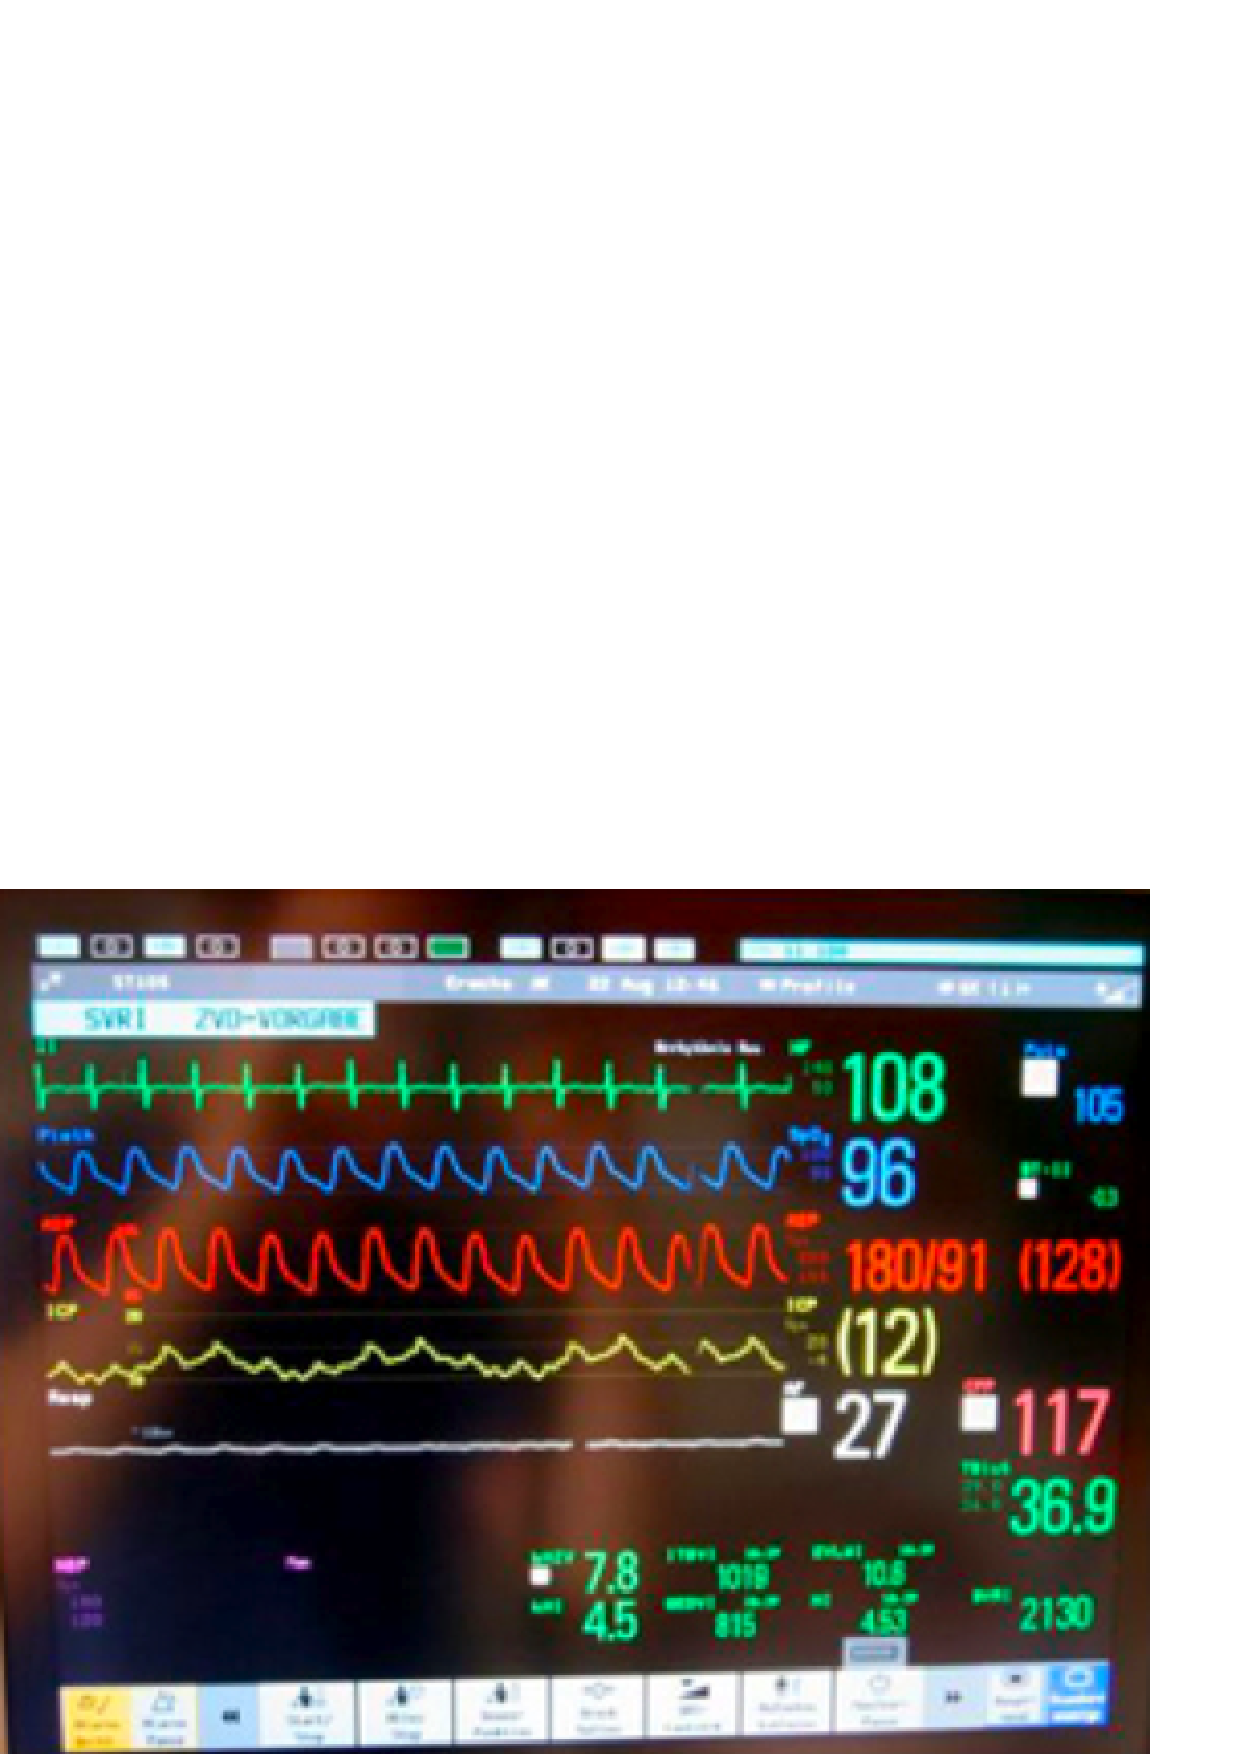
\includegraphics[width=0.6\textwidth]{micu-screen}
   \caption{An example medical ICU screen.}
   \label{fig:micu-screen}
\end{figure}

\begin{figure}[htbp]
   \centering
   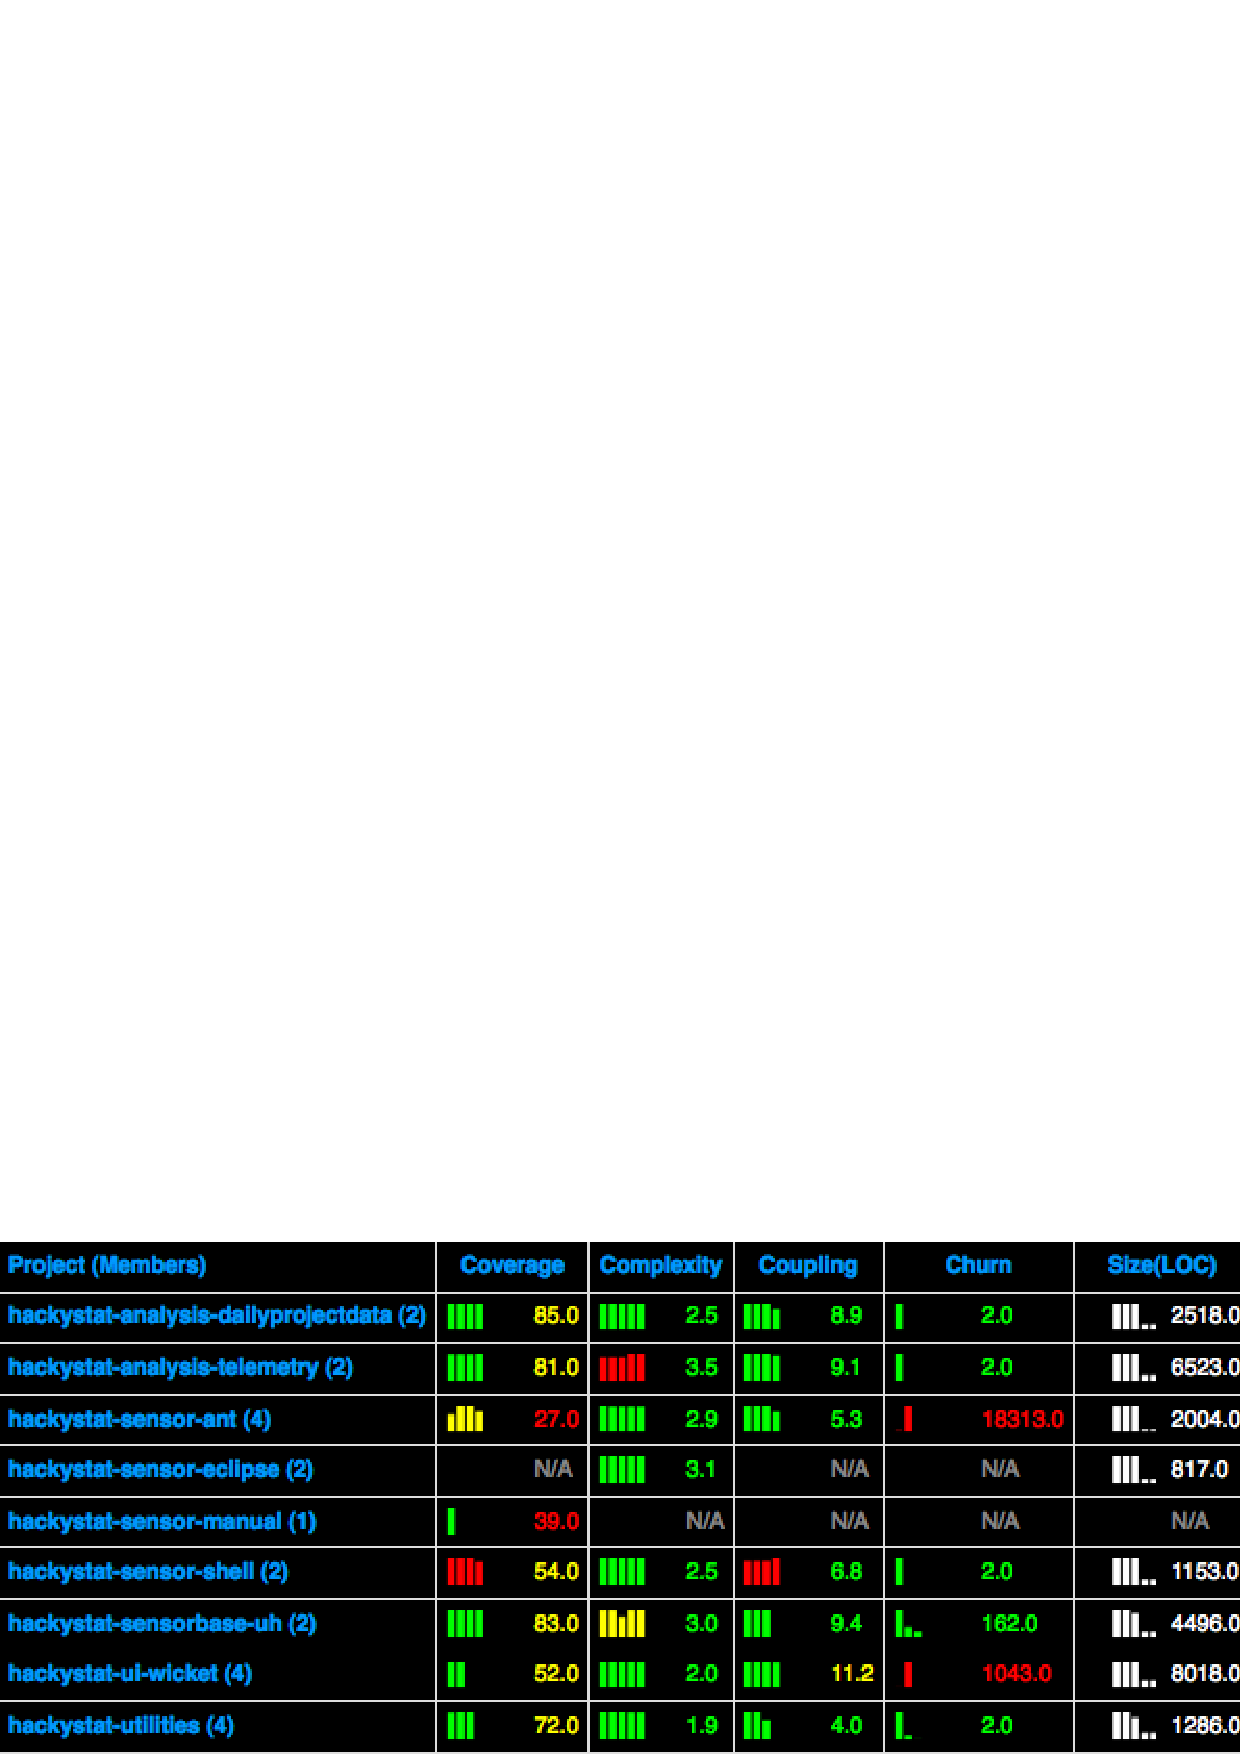
\includegraphics[width=\textwidth]{SICU}
   \caption{An example Software ICU screen.}
   \label{fig:SICU}
\end{figure}


In the Software ICU, software metrics are used as vital signs, and are monitored intensively. The ``health'' states of the software are determined, and marked with color, so that developers can plan ``treatment'' for their software project accordingly. \autoref{fig:SICU} illustrates an example Software ICU screen. Each metric represents a factor in software development process. When a metric departs its reasonable behavior, it indicates that a factor of the software development process might go wrong. ``Treatment'' is required to fix that in order to avoid possible project failure.
 
Similar to medical ICU, Software ICU's vital signs are presented with both historical trend and current state, each of which is then colored separated. Different vital signs may use different coloring methods and parameter configurations. Unlike the medical ICU, whose vital signs (temperature, respiration, etc.) have been studied in some cases for hundreds of years, no comparable body of research exists in software engineering on how to intensively monitor multiple software measurements to determine the state of software project or how different behavior of metrics impacts upon the state of software project. Therefore, my selection of vital signs and their configurations are research hypothesis, and are validated in the case study.

\section{Evaluation of Software ICU}
Undergraduate students enrolled in a Software Engineering course assisted with the evaluation of this research. The class consists of 18 students. In the second half of the semester, they were divided into 5 groups and developed two course projects. Hackystat and Software ICU were introduced to the class to help them understand the health state of a software project. 

They used the system for approximately six weeks, and their activities on the system were logged during that period. At the end of the semester, the students were invited to participate in a survey that asked their opinion of Hackystat and Software ICU.

I compared and analyzed the result from system logs and questionnaire responses to find out how they used the system and what impact the system had on their development.

\section{Thesis Statement}
This research investigates the mechanism and technology of Software ICU and gathers data to assess the following hypotheses: 
\begin{enumerate}
\item Adopting metaphor of medical ICU to software engineering is practical and feasible.
\item The selection of vital signs is appropriate.
\item The coloring mechanism correctly illustrates the health state of the vital signs.
\item Knowledge of health state of their projects helps students improve their performance in collaborative software development.
\end{enumerate}
The first hypothesis claims that it is possible to implement an application that monitors multiple software development measurements and can be used to direct software development practice in a way similar to medical ICU.

The second hypothesis claims that the selection of vital signs is adequate to reveal potential defects during software development.

The third hypothesis claims that with a decent coloring method, the vital sign of different conditions will be assigned different colors, and the same color can be traced back to similar conditions.

The fourth hypothesis concerns a chain reaction of events. When students know the health state of the vital signs of their projects, they will need to fix their code or improve their development practice if the vital sign is not healthy. By trying to keep vital signs healthy, students should discover better ways to collaborate with other teammates and produce high-quality software.

\section{Thesis Structure}
The remainder of this thesis is as follows. Chapter 2 presents some previous studies related to this research. Chapter 3 describes the Hackystat system, which Software ICU is built upon. Chapter 4 contains detailed description of the design and implementation of Software ICU. The evaluation procedures are described in Chapter 5 and the results are discussed in Chapter 6. Finally, Chapter 7 contains the conclusions and future directions of this research. 



\chapter{Related Work}
This chapter presents some work related to my research.

The first part discusses previous research on empirical software engineering concepts. Most previous research on measurement-based software engineering focuses on methodology. Effective approaches are developed and deployed in actual practice. However, the lack of automation adds significant overhead to developers, thus leading to the impression that they are hard to do. Research on Hackystat and the Software ICU is oriented towards a new generation of approaches to PSP metrics that automate data collection and analyze\cite{csdl2-02-07}.

The second part discusses three recent research projects that focus on automated data collection. Two of them mainly focus on introductory level programming courses and are not very suitable to senior software development or professional settings. The third one is very similar to Hackystat and has related industry studies.

%Third part discusses some commercial ``dashboards'' for software project data. Software ICU is one example of a project dashboard. However, it differs from commercial approaches with its intensive metrics, high extensibility and open source development and distribution. 

The last part discusses two previous related case studies of the Hackystat system to provide some insight into the use of Hackystat in a classroom setting prior to the use of the Software ICU.

\section {TSP/PSP}
The Personal Software Process (PSP)\cite{book:psp} and the Team Software Process (TSP)\cite{book:tsp} are among the most extensively studied approaches for measurement-based software engineering. They were developed by Watts Humphrey to teach students (in university and industry alike) about the use of large scale methods based on the Capability Maturity Model (CMM)\cite{cmm}. The PSP attempts to scale down industrial software practices to fit the needs of small scale program development. Software processes and software engineering disciplines are gradually introduced through small program projects (e.g. course assignment projects). The PSP maturity progression is shown in \autoref{fig:PSP-Evo}. Students gather both process and product measures on a set of projects. By comparing the measurement result to their original planning, they gain insight into their programming habits, both pros and cons, and improve their process to higher level of maturity.

\begin{figure}[htbp] %  figure placement: here, top, bottom, or page
   \centering
   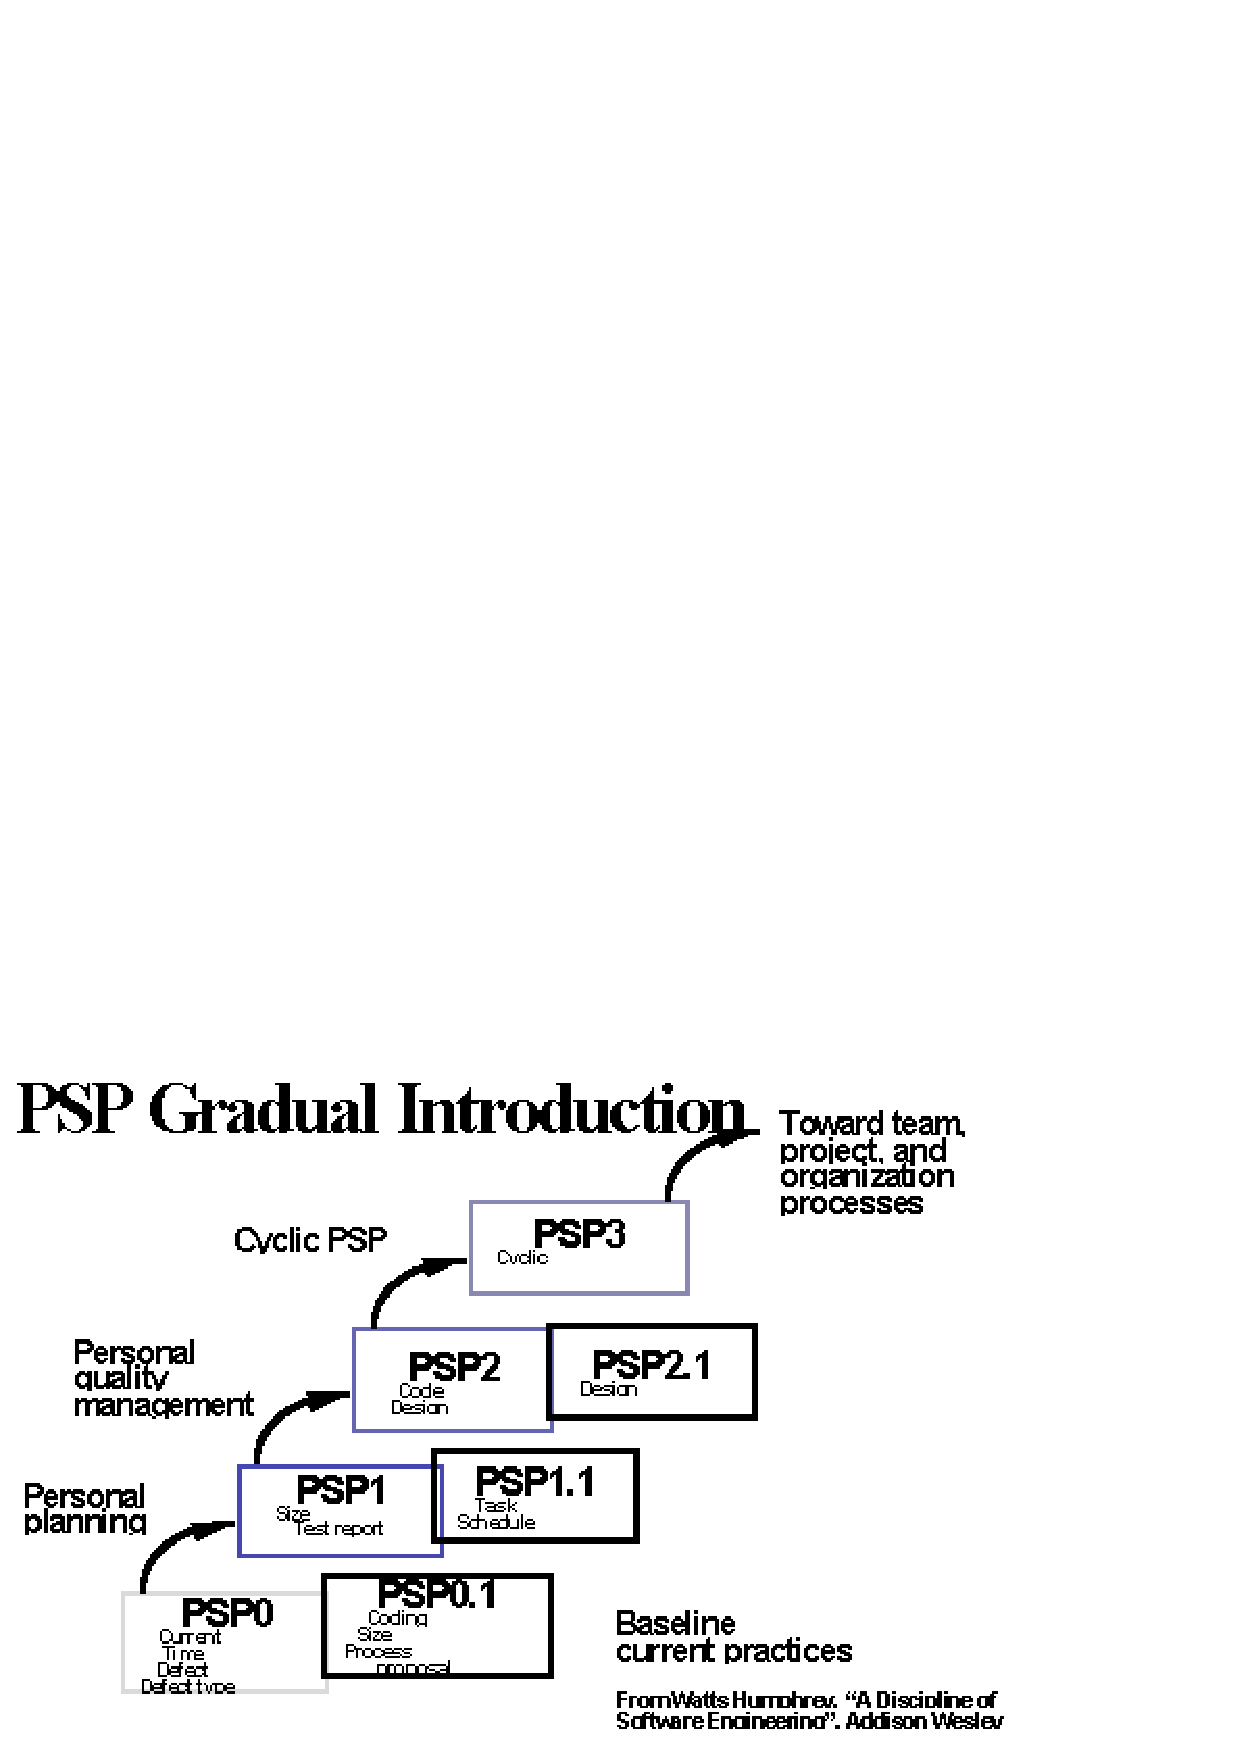
\includegraphics[height=20em]{PSP-Evo} 
   \caption{Progression of PSP}
   \label{fig:PSP-Evo}
\end{figure}

%PSP/TSP is effective in both academic education as well as industrial application. (more about related research)

A major drawback of the PSP is lack of automation. Developers have to manually record their process and product data (mostly the development time and number of defects). The high overhead of data collection raises a barrier to its introduction and adoption. Additionally, it is not easy to ``digest'' the data. Developers have to manually analyze their logged data in order to understand the their performance, then be able to improve it.

On the contrary, Software ICU explores how one can provide a higher level of automation in tracking and analyzing software process and product data.


\section {Research Based on Automated Data Collection}
Project ClockIt and Retina are two recent research projects based on automated data collection to support entry-level programming courses, while PROM is the most similar research to Hackystat.

\subsection {Project ClockIt and Retina}
Project ClockIt provides a data logger as a BlueJ\footnote{``BlueJ is an integrated Java environment specifically designed for introductory teaching.'' --Quoted from \url{http://www.bluej.org/about/what.html}} extension. It records developer's open/close of project and package events, file change and delete events and compilation results. Data is saved to a local file and later sent to a database via the Internet. A data visualizer integrated into BlueJ is available to view data about the current project. \autoref{fig:clockit} shows an example of this visualizer. Data stored in database is used for statistic analysis such as class averages. A web interface is also available to instructors to view the individual data of their students and class average analysis data.

\begin{figure}[htbp] %  figure placement: here, top, bottom, or page
   \centering
   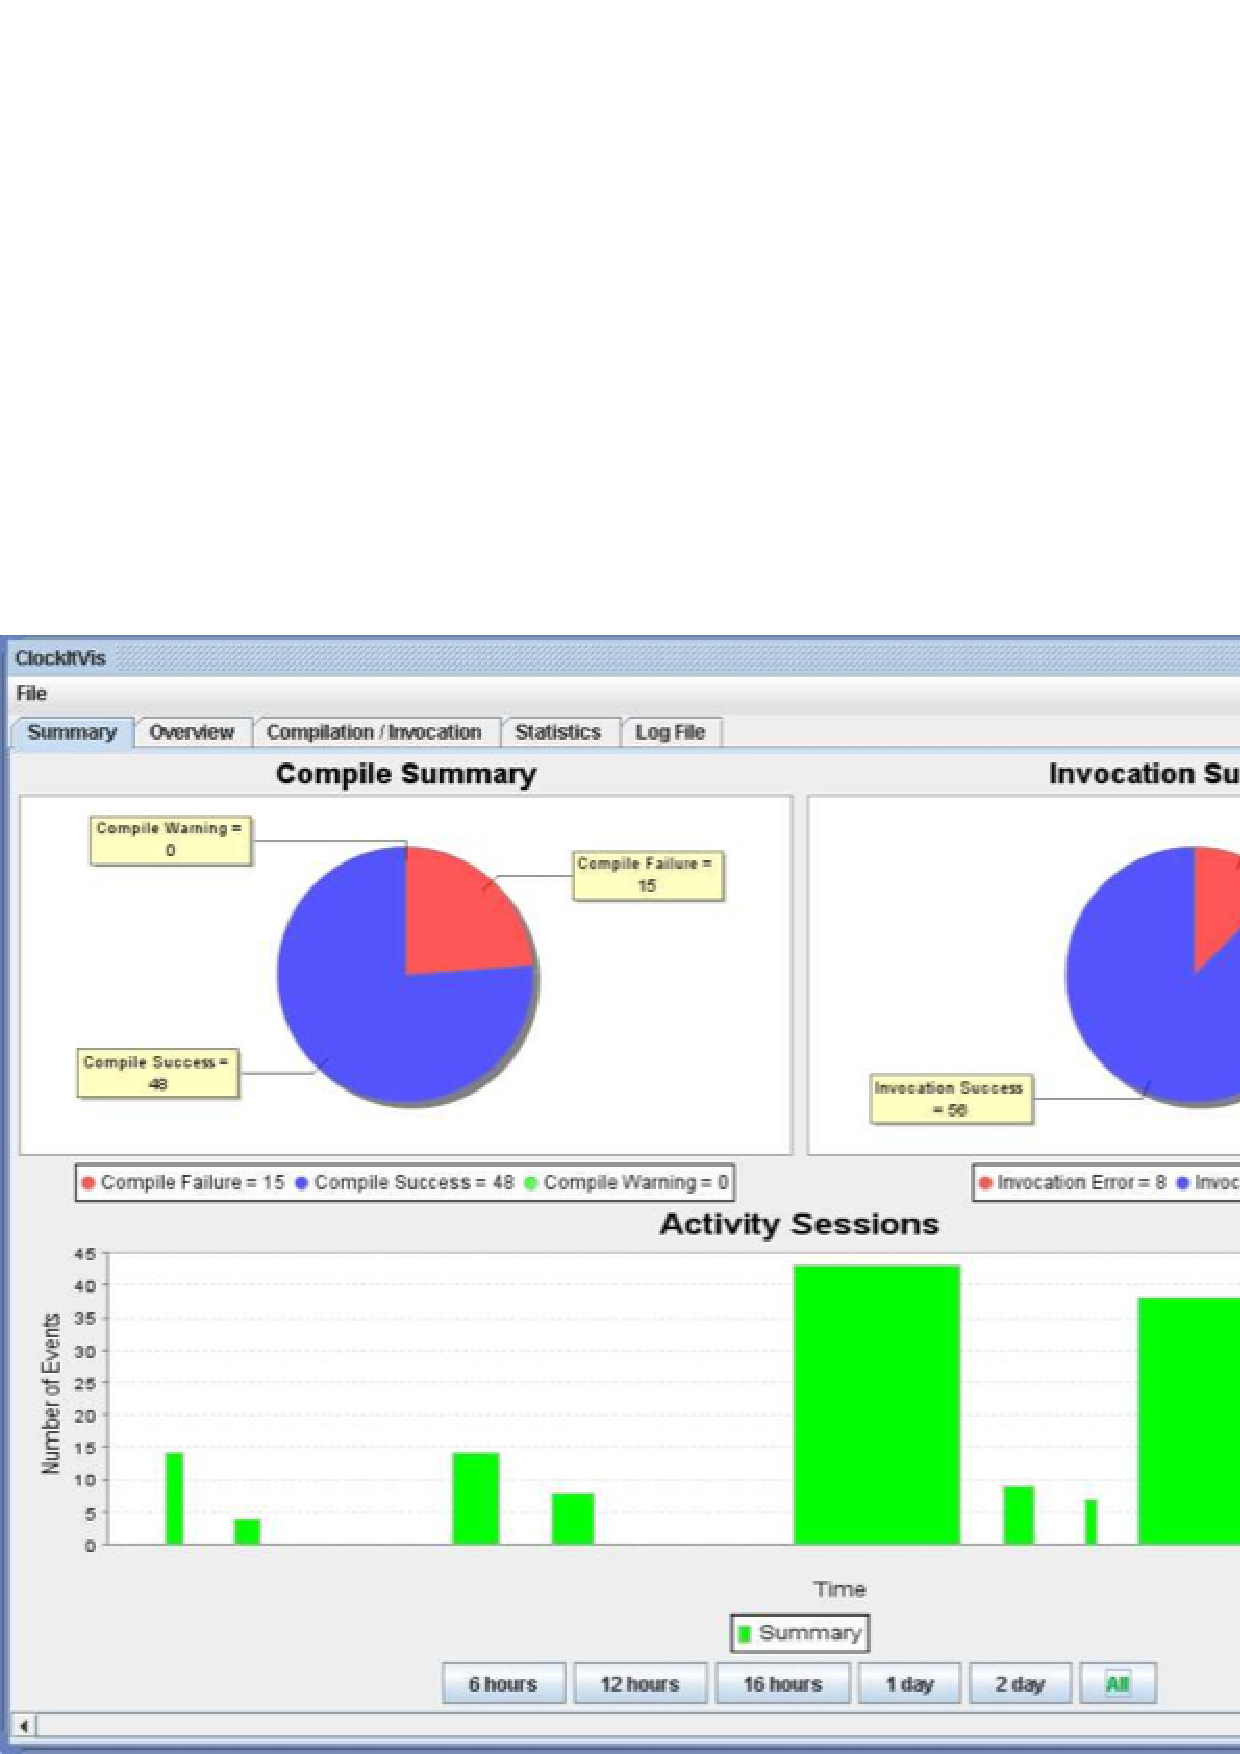
\includegraphics[height=20em]{clockit} 
   \caption{ClockIt BlueJ Data Visualizer summary}
   \label{fig:clockit}
\end{figure}

Closely related to ClockIt, Retina also provides automated data collection. Though Retina provides more tool support (BlueJ, Eclipse and command-line compiler), it focuses on a even smaller area of programming events: compilation. It gathers data from students' compilation events, mostly compilation errors. In additional to its data viewer (see \autoref{fig:retina}), it also provides a recommendation tool for students. The tool uses instant messaging (IM) to give students an estimate of the amount of time required for the upcoming assignment, and the compilation errors one is likely to make. These are based on both the student's previous data and the data from courses of previous semesters. 

\begin{figure}[htbp]
     \centering
     \subfigure[Retina Instructor Viewer]{
          \label{fig:retina-teacher}
          \includegraphics[width=.48\textwidth]{retina-teacher}}
     \subfigure[Retina Student Viewer]{
          \label{fig:retina-teacher}
          \includegraphics[width=.48\textwidth]{retina-student}}
          
     \caption{Data viewers of Retina.}
     \label{fig:retina}
\end{figure}

The difference between these two research projects and the Software ICU is that ClockIt and Retina focus only on introductory level courses, where compilation is the interesting development event. On the other hand, their relatively easy configuration contrasts with one of the major short-comings of Hackystat and the Software ICU. As neither of them provide good extensibility, they are unlikely to be useful in advanced programming situations like advanced programming course or professional setting.

\subsection {PROM}
PRO Metric (PROM) \cite{prom03} is a system that is quite similar to Hackystat. PROM is a software system for collecting process and product metrics in a software company. It is initiated and driven by the demand of the company, and thus the research focus is on an industry setting. It is designed to work fully automatically without any interaction with the user in order to get reliable and accurate data about company internal workflows and development processes. It is organized in a sequence of interconnected components, communicating using the SOAP protocol. Similar to sensors in Hackystat, it has plugins to collect data for many different applications, including IDEs, word processing tools, email clients, and issue tracking systems. Data then is transmitted to a plugin server to extract metric, then the results are sent to PROM server to store into database. \autoref{fig:promarchitecture} shows the overview of PROM's architecture.

\begin{figure}[htbp]
     \centering
     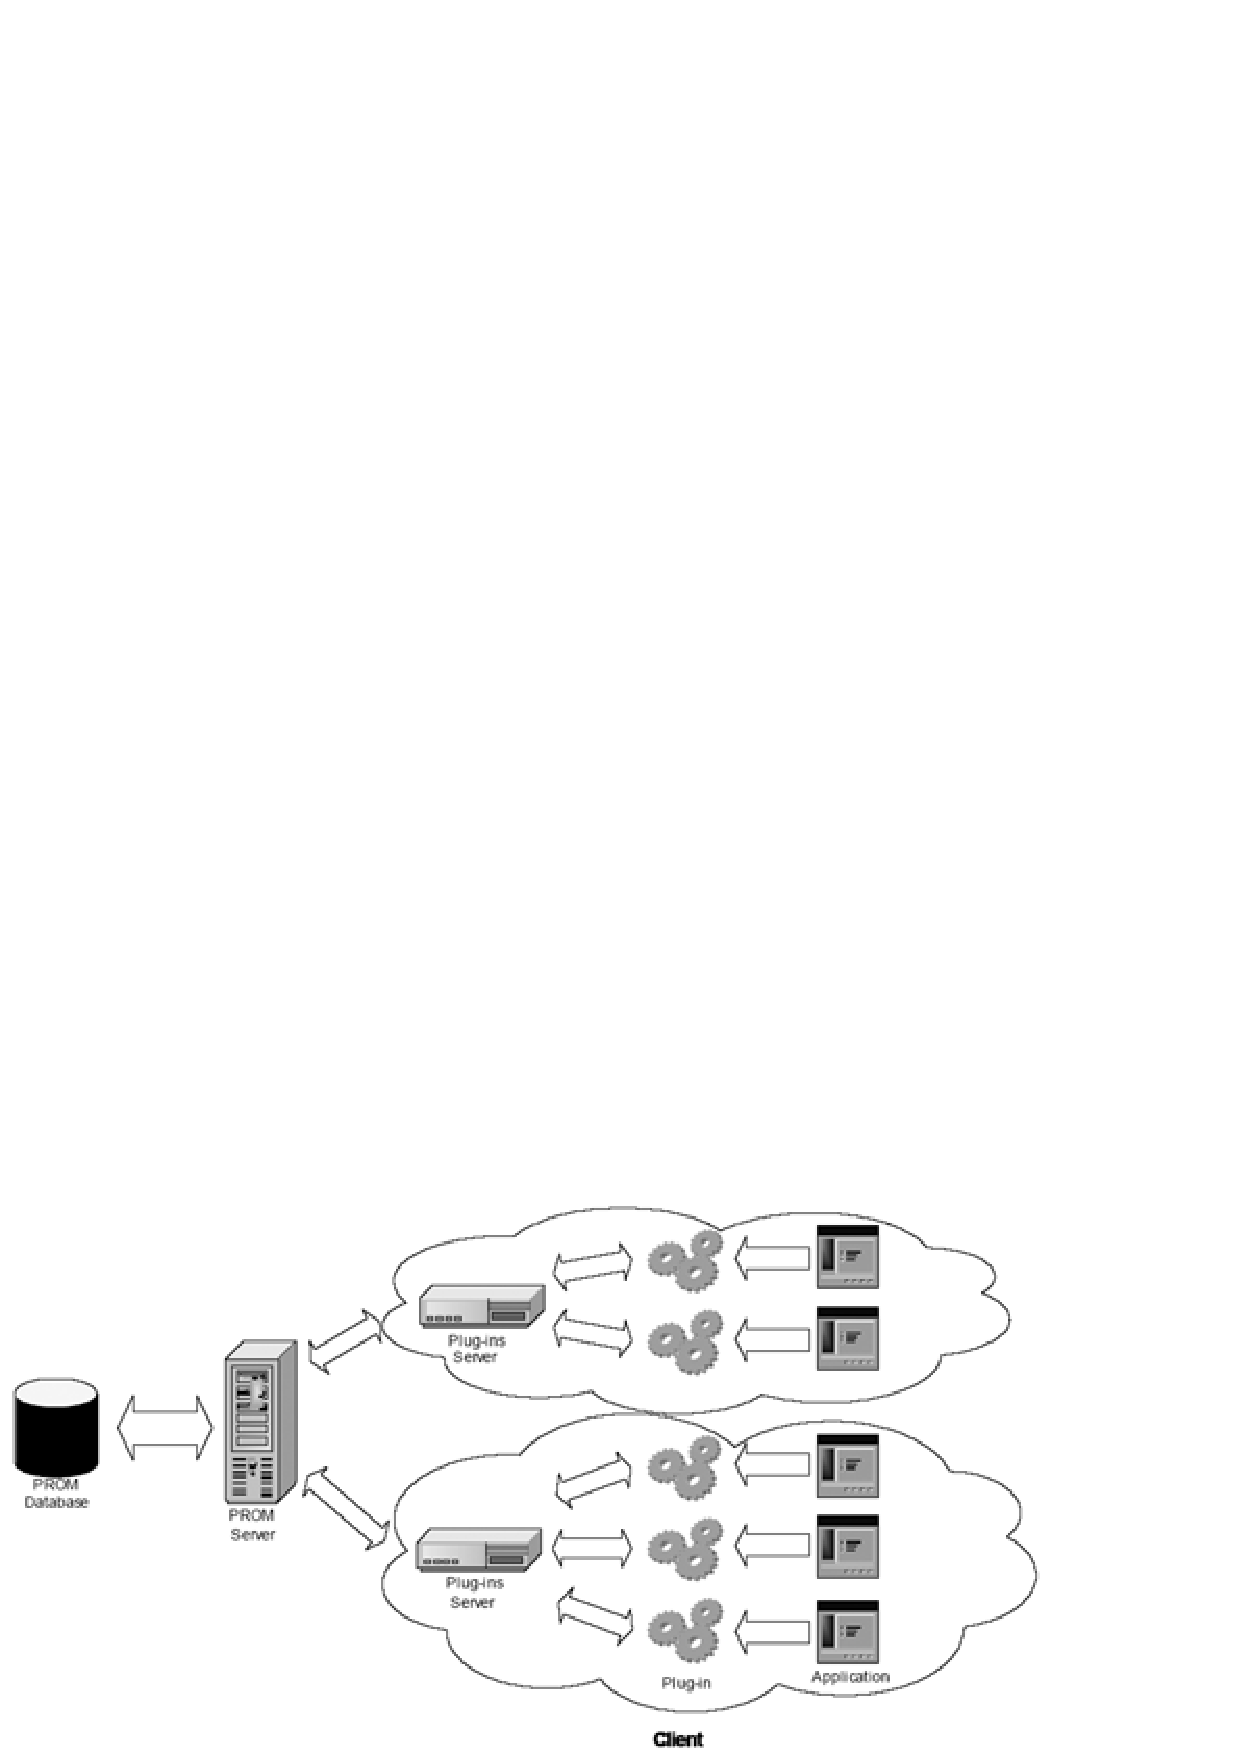
\includegraphics[width=.48\textwidth]{promarchitecture}
     \caption{Architecture of the PROM system}
     \label{fig:promarchitecture}
\end{figure}

PROM categorizes users into 3 roles, developer, team leader, and manager of the team. Each of these roles is provided with different views of the data. Developers have access to their individual, detailed data, the leader has access to the aggregated data of the whole team, and the manager has access to project level aggregated data.

Compared to Hackystat, PROM's data is stored as analyzed metrics results while Hackystat stores the raw sensor data. The disadvantage of storing raw data is that, analysis has to be executed each time the results are requested, while the advantage is that the abilities to modify analysis algorithms and to run new analysis on existed data are retained. Moreover, Hackystat's caching mechanism compensates the disadvantage to some extent. In PROM, different data viewers are provided to different groups of users while Hackystat does not restrict views based upon the role of a member on a project.

A recent case study of PROM in an industrial environment\cite{prom09} discusses the lessons learned from two years experience of using the PROM system in the IT department of a large company in Italy. Evidence indicates that adopting a system like PROM requires a long set-up phase and needs the company and development team's patience and commitment to succeed, but it can eventually delivers value to the company. 

One of the lessons suggests that data presentation is as important as data accuracy and simplicity, brevity and clarity is preferable. Another lesson suggests that fast aggregated view of data is desired, and users of different roles favor different aggregations, e.g. developers like reports of their daily activities, while team leader and manager like summary views of data on team and project level. The Software ICU's simple and fast data presentation and high configurability and extensibility would appear to address these requirements.

%\section {Software Project Dashboards}
%In software industry, there exists many commercial software project manage dashboards, such as LightHouse, ProjectManager.com dashboard, PivotLink Dashboards, Autotask Project Management and so forth. However, many of them are complete solution of software development business management, including not only software project states management, but also related resource allocation and budget control, etc. As being commercial products, they are not open source. Most importantly, there is few research published about these commercial project dashboards. ``Features'' are advertised as other commercial products, while short-comings are ignored. Thus negative results of their use are unknown. This research of Software ICU contains not only its benefits, but also its negative impact.


\section {Previous Case Studies of Hackystat}
The classroom study presented in this thesis is the third case study of the Hackystat system in a classroom setting. 

The first case study was performed in 2003 used an early version of Hackystat\cite{csdl2-03-13}. During that time, Hackystat was only collecting 4 types of metrics (Active Time, Size, Unit Tests and Coverage). The system was oriented around a set of ``Course'' analyses that were tailored to an educational setting. Those analyses summarized the individual team project metric data in tabular form, and also presented comparisons of all of the course projects (\autoref{fig:hackystat2003}). The case study evaluation showed that the installation of Ant sensors is the most significant barrier to the system. It was too difficult to install without direct help from the development team. But the overhead of use is relatively low and analyses were usable and useful. However, the lack of data privacy was uncomfortable for some students.

\begin{figure}[htbp]
   \centering
   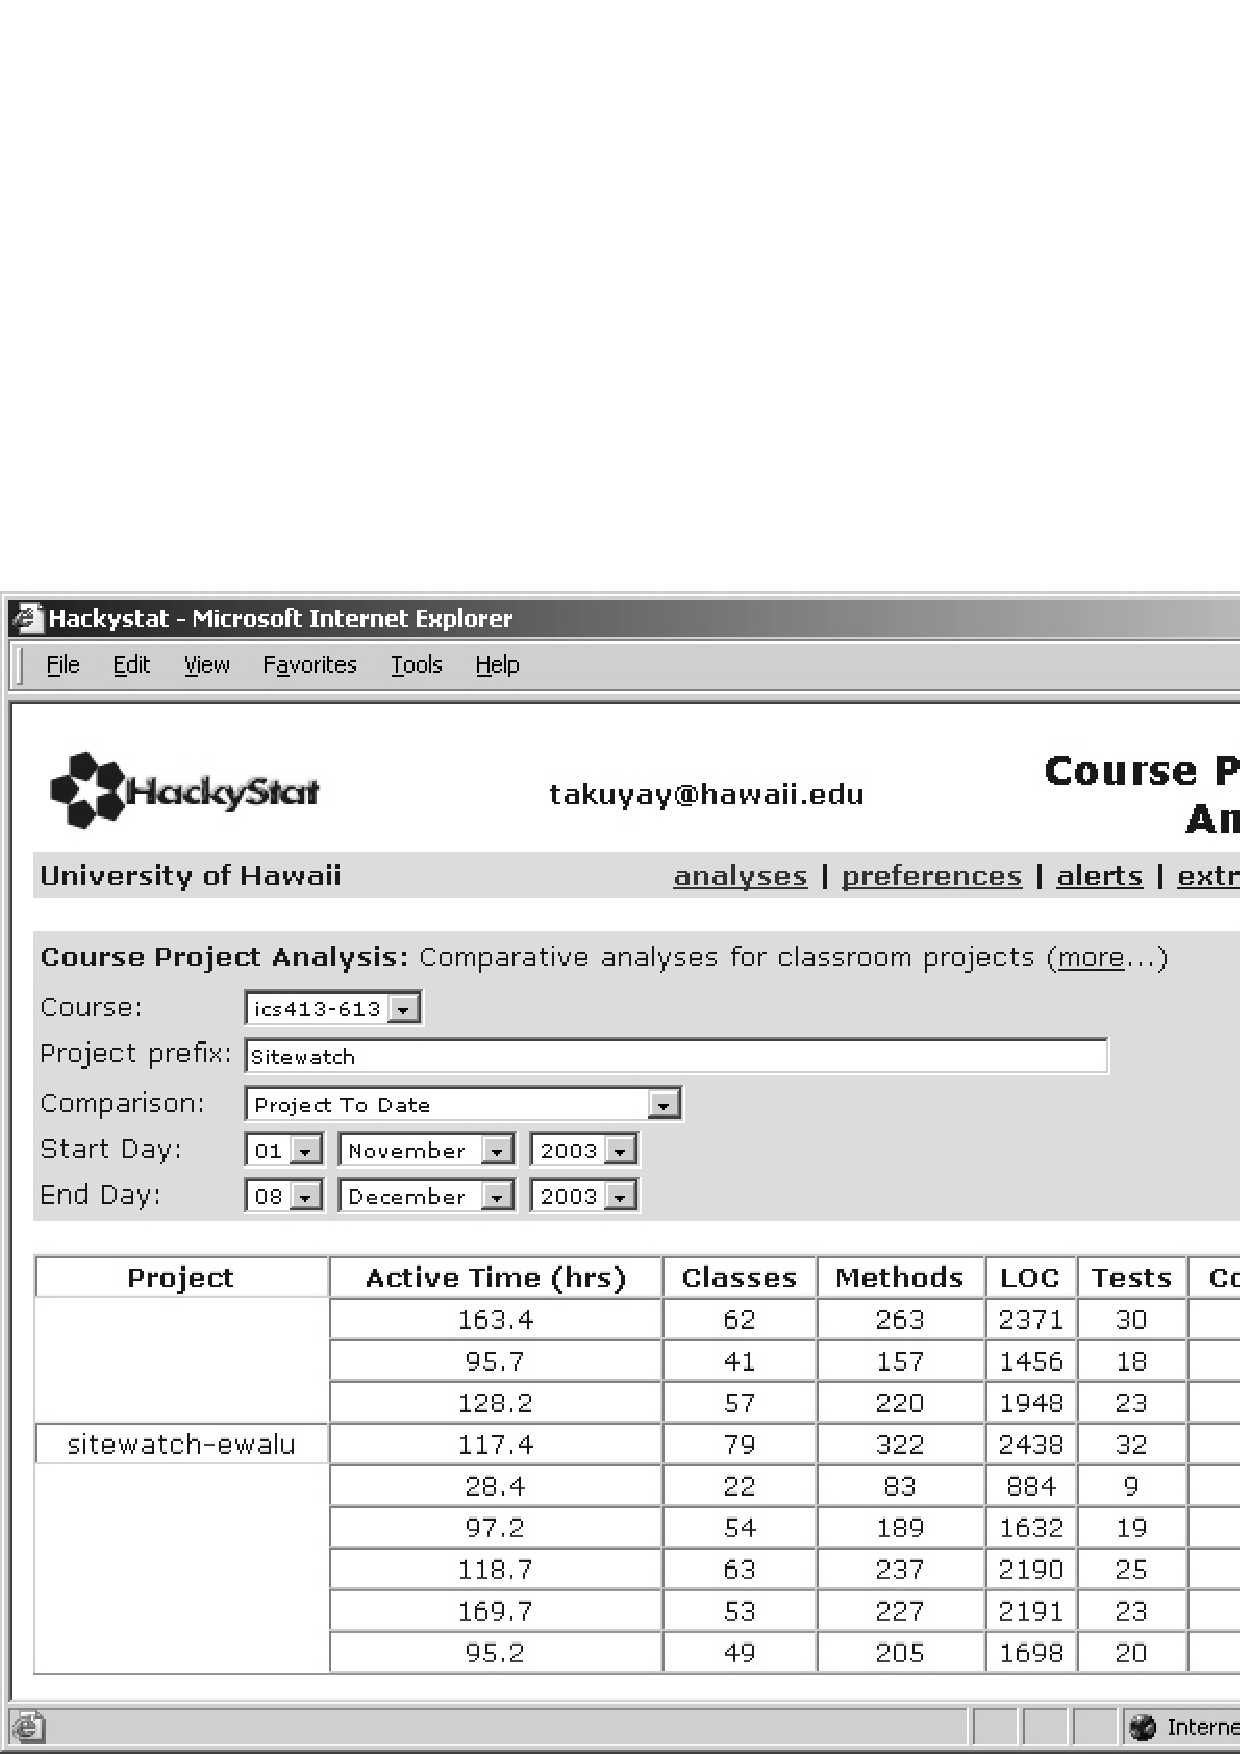
\includegraphics[height=20em]{hackystat2003} 
   \caption{Screenshot of course project to date analysis of Hackystat in 2003}
   \label{fig:hackystat2003}
\end{figure}

The second case study was performed in 2006 as a partial replication of the first case study\cite{csdl2-07-02}. Hackystat had undergone significant change from 2003 to 2006. The sensor installation, which is the major barrier to the system in 2003, was automated by the hackyInstaller GUI, which greatly lowers the overhead of configuration for developers. The evaluation confirms this with a substantial drop in sensor installation difficulty. However, a new sophisticated Telemetry analysis \autoref{fig:hackystat2006} and its complex user interface raised the difficulty of using it and interpreting data, leading to slight drop in usability and professional feasibility.

\begin{figure}[htbp]
   \centering
   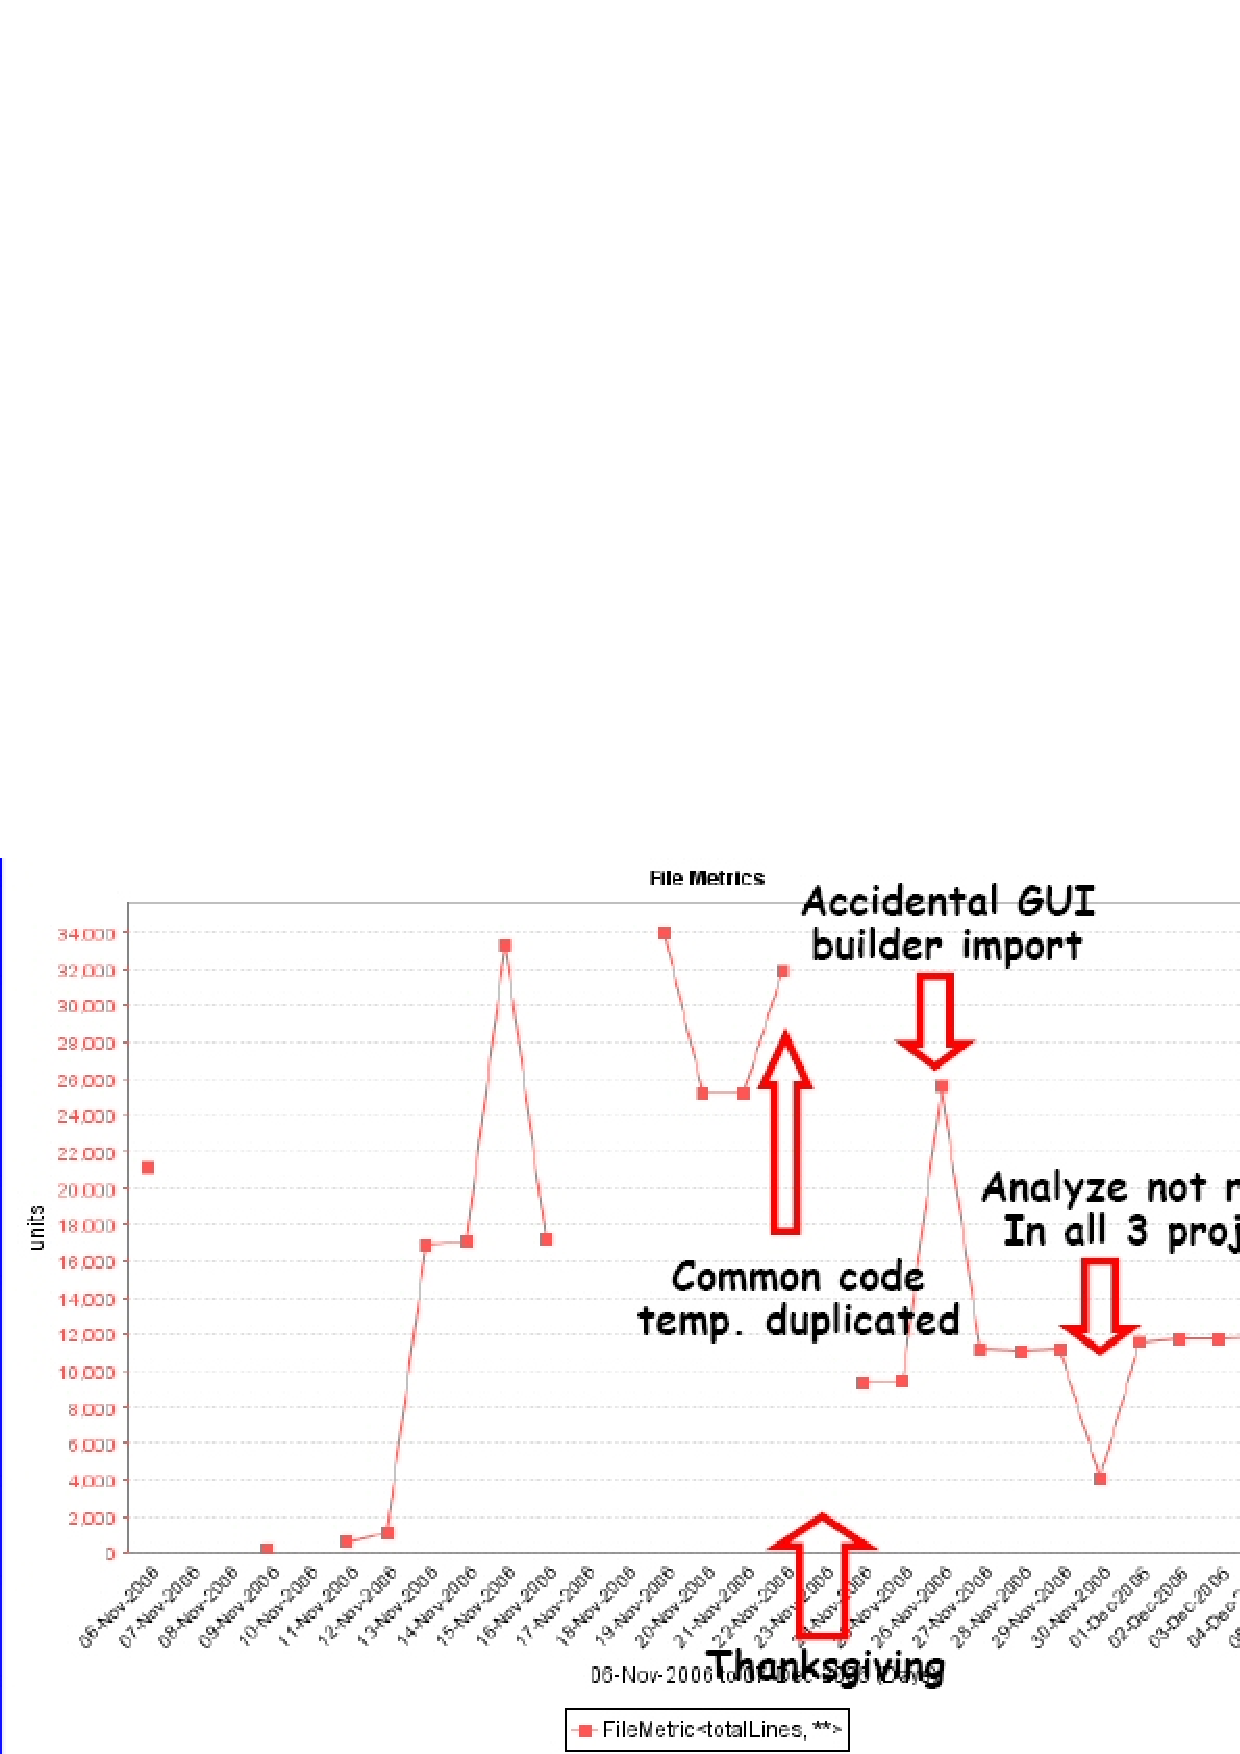
\includegraphics[height=20em]{hackystat2006} 
   \caption{Screenshot of file-metric telemetry analysis of Hackystat in 2006}
   \label{fig:hackystat2006}
\end{figure}

In 2007, Hackystat was re-implemented with a new architecture. Adopting a service-oriented architecture enables the development of multiple user interfaces separate from the data collection and analysis components. The Software ICU is built upon a new web-based UI called Project Browser, and the classroom study is also based on this user interface.


\chapter{Hackystat}
In this research, the Software ICU is built upon Hackystat to fulfill automated data collection and analysis. This chapter briefly describes the Hackystat system, which was invented by Professor Philip M. Johnson, in the Collaborative Software Development Laboratory, Department of Information and Computer Sciences, University of Hawaii at Manoa. 
 
\section{Hackystat Framework}
Hackystat is an open source framework for collection, analysis, visualization, interpretation, annotation, and dissemination of software development process and product data. Hackystat consists of many software services that communicate using REST architectural principles\cite{rest}. These software services can be categorized into 4 groups: sensors, data repository, analysis services and viewers. \autoref{fig:hackystat-architecture} shows the architecture of Hackystat system. 

\begin{figure}[htbp]
   \centering
   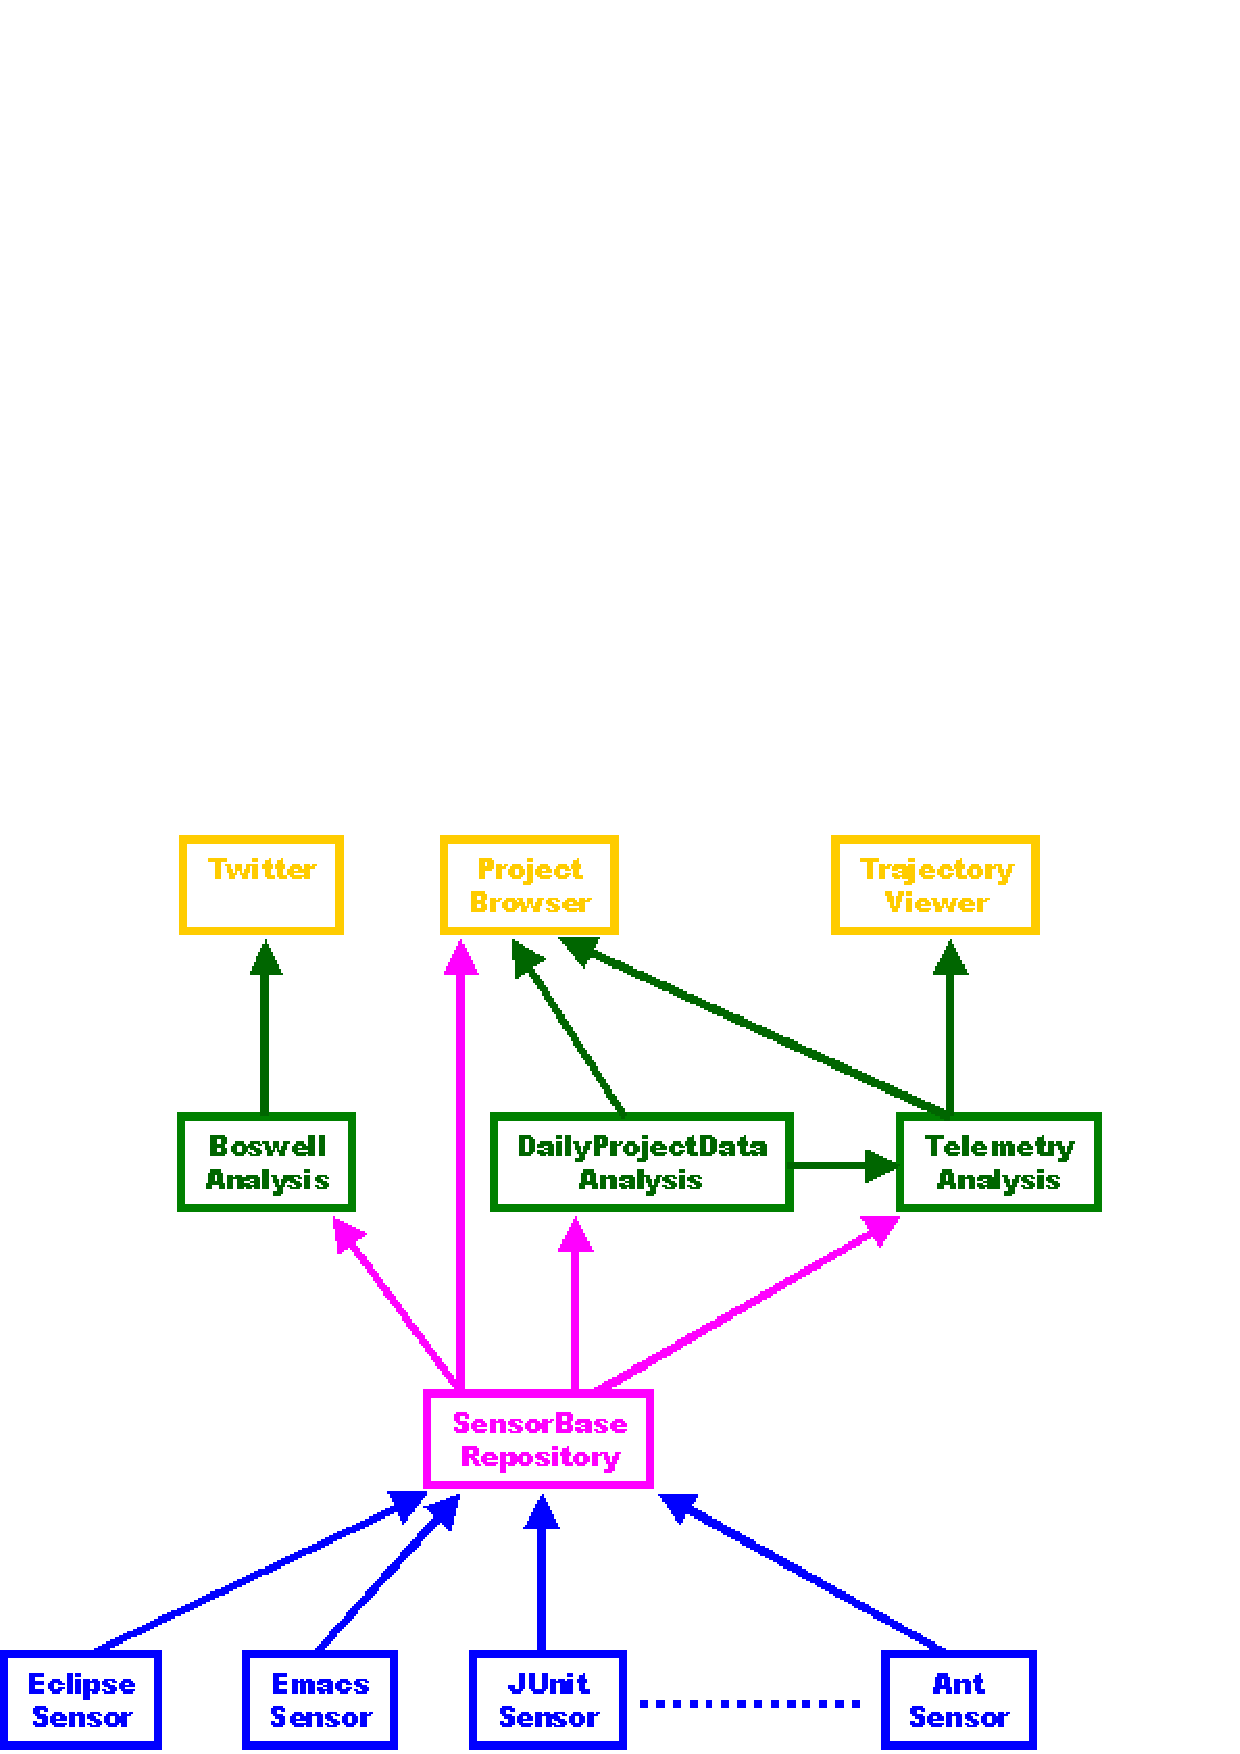
\includegraphics[height=20em]{hackystat-architecture} 
   \caption{Architecture of Hackystat}
   \label{fig:hackystat-architecture}
\end{figure}

\subsection{Sensors}
Sensors are small software plugins that collect data from the use of tools and applications. Currently, sensors are available for many development software systems including Eclipse, Emacs, Ant, etc. Sensor data is represented in XML, and consist of seven basic elements: data owner, resource, timestamp, runtime, tool, Sensor Data Type and properties. The first six are required and the last one is optional. 

The Sensor Data Type(SDT) is specified for every piece of sensor data when collected, so that the same type of data can be collected from different tools and higher level services can easily determine which data is relevant to them. Sensor data is designed to record only an piece of atomic data such as size of a single file. The runtime field is used to group data that belongs to the same event, such as the file metrics associated with a project. Properties are additional information for different types of sensor data, such as coverage value for coverage SDT and lines of code for file metric. 

Sensors are designed to work automatically without any attention from the user apart from initial configuration. In order to reduce internet communication and support offline work, data is temporarily stored locally, then sent to the data repository every several minutes or when internet connection is available.

\subsection{SensorBase}
Sensor data is sent to the data repository, called the SensorBase. The SensorBase stores the data as it is sent from sensors, and provides RESTful interface for easy manipulation of the data using HTTP. Sensor data can be queried with the six required elements mentioned above via HTTP calls, and data is sent back as XML. The SensorBase is implemented with a database manager abstract class, thus it is easy to add support for different database implementations. The current version of Hackystat provides database support for Derby, Oracle and PostgreSQL.

\section{Analysis Services}
The analysis services of Hackystat provide abstractions of the raw data from SensorBase. DailyProjectData and Telemetry are the two most fundamental analysis services of Hackystat.

\subsection{Daily Project Data Analysis}
As its name indicates, DailyProjectData (DPD) service provides abstractions of sensor data associated with a single project within a 24 hour period, which represents a simple software development metric on a single day. Data for a single project includes data from all members of that project. In a DailyProjectData instance, both a summary value, e.g. total development time across the project, and detailed values, e.g. total development time of a project member, are available. So it is easy for higher level services to use this data.

Each DPD analysis generates software metric from data of a certain Sensor Data Type. Current available DPD analyses are Build, Code Issue, Commit, Complexity, Coupling, Coverage, Dev Time, File Metric, Issue, and Unit Test. These DPD analyses are the basis of the Hackystat system, most other analysis services are based on DPD. While DPD is a low level of abstraction, these can also be considered as the available software metrics in Hackystat.

\subsection{Telemetry Analysis}
Based on DPD service, the Telemetry service provides abstraction over a longer period of time such as several days, weeks or months. A Telemetry Chart consists of one or more streams of data points. Each data point represents the metric value of in a single granularity (day, week or month). Together they show the trend of the metric(s).

There is a special group of Telemetry charts called Member-Level Telemetry. These charts consist of several stream, each of which belongs to a project member. They are used in Software ICU's drill down feature to compare performance of each member within a project. 

To support the work practices of different organizations, Telemetry service provides a domain specific language that allows to build new Telemetry Chart with Telemetry stream lines. The predefined Telemetry Charts are all written with this language.

Telemetry streams can also accept parameters to refine the object data. This feature is inherited in Software ICU, where user can configure the parameters of each Telemetry analysis of each vital sign (more detail discuss in \autoref{vitalSign} and \autoref{SICUconfiguration}).

\section {Project Browser}
Project Browser is one of the viewers in Hackystat system. It is based on Wicket\footnote{\url{http://wicket.apache.org/}}, a Java-based web application framework. Project Browser is integrated with viewers to all Hackystat services, which are organized as tabs. 

With the help of Wicket's modularization, viewers on Project Browser can share common panels, such as project/date selection panels and Ajax loading process panel, which facilitate the development of new pages. This also makes user's experience more consistent across different viewers. Therefore it now serves as a data presentation and high level analysis development center. Several new presentations and high level analysis are developed upon it. The Software ICU is one of them.




\chapter{Design and Implementation of The Software ICU}
In order to utilize multiple software development metrics to manage software development process, I adopt the metaphor of the medical ICU and develop a system called the Software Intensive Care Unit (Software ICU). It consists of a set of vital signs, each of which is based on one software development metric and indicates the project's ``health'' state from one perspective.

\section{Interface of Software ICU}

The interface to the Software ICU is separated into two parts. The left-hand side is the control panel, where the user can pick the analysis period, data granularity and selected projects to analyze. The right-hand side consists of three panels: the data panel, the loading process panel, and the configuration panel. Each of these panels is discussed in following sections. The data panel is the major panel that shows the result of SICU analysis. \autoref{fig:overview} shows an example of Software ICU.

\begin{figure}[htbp]
   \centering
   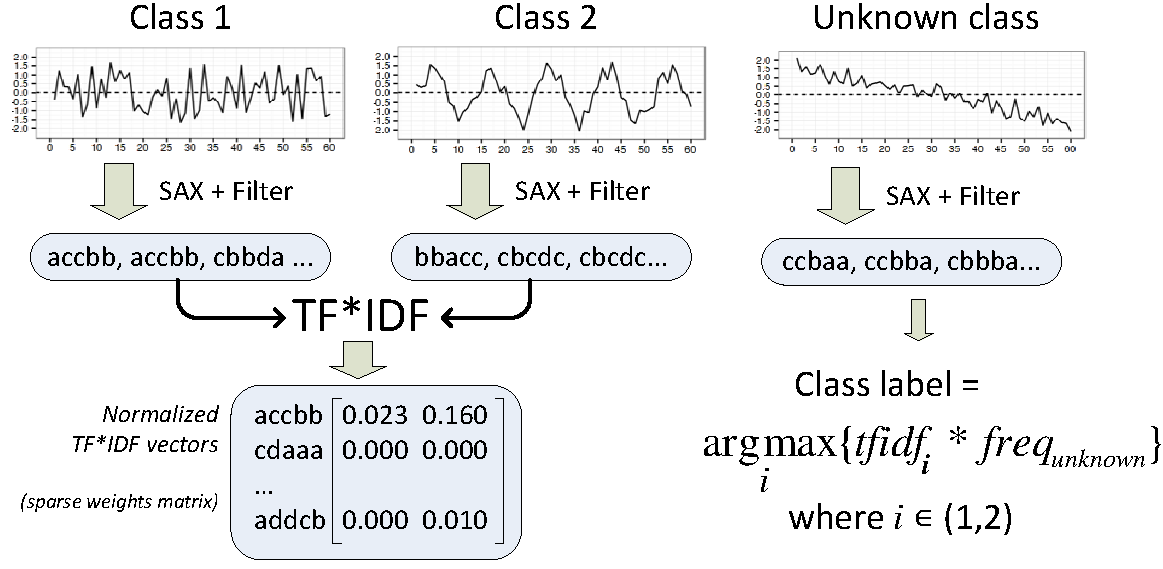
\includegraphics[width=\textwidth]{overview}
   \caption{A screenshot of Software ICU}
   \label{fig:overview}
\end{figure}

\section {Definition of Related Terms}
Before the discussion of the design of Software ICU, two terms are needed to be clarify. 

``health''

``vital sign''

\section{Vital Signs}
\label{vitalSign}

Similar to the medical ICU, the use of multiple software development metrics in Software ICU is necessary because there is not a single metric that can determine the health state of a software project. Similar to medical vital signs, each software metric shows different aspect of a software project. Changes in one of them may or may not indicate a change in the overall health state, but changes in more of them indicates a higher possibility that health state changed. In this study, we use nine vital signs in the Software ICU.

Vital signs of software projects are measured by various software development process or product metrics. Each of these vital signs reveals an aspect of the health state of the software project. In this section I will discuss all these vital signs.
\begin{description}
\item[Coverage] 
Coverage is a good indicator of the tests' quality. It stands for the test coverage of source code in unit testing, which is usually measured as the percentage of code units (line, method, class, etc) that is executed during testing. There are a number of coverage criteria, such as line, method, class, conditional, etc. In the Software ICU, the user can select which to use. No matter which criteria is chosen, higher coverage is always better because a higher percentage of code covered by unit testing indicates a lower risk of defects in the untested code. However, high coverage does not necessarily mean good quality unit test, or vice versa. One reason is that, in some situations, it is difficult to achieve high test coverage because of the difficulty of verifying results, especially when using UI frameworks. Another reason is that the code executed during unit testing can be unverified. For example, when testing an image processor with a given image file, the code of loading the image file is executed, but the test does probably not have assertion about the correctness of loading the file. But as long as developers don't have the intent to trick coverage in order to pretend to be writing enough unit tests (which is possible if coverage is misused to judge their performance), raising coverage is always a good thing.

\item[Cyclomatic complexity] 
Cyclomatic complexity, a measurement of the complexity of a program developed by Thomas J. McCabe, measures the number of linearly independent paths through a program's source code\cite{mccabe:complexity}. The higher the cyclomatic complexity, the more distinct control paths exist in a program module, and the more difficult it is to achieve high path test coverage. Additionally, code of high complexity is often difficult to understand, thus it is hard to maintain. Therefore, program modules  with low complexity are preferred. But high complexity is not necessarily evil. The nature of some programs just requires a high level of complexity. Also a raise in complexity is sometimes unavoidable during development, especially when optimizing code performance. However, developers should try to avoid high complexity unless it is necessary, especially in early stages of development, so that the code is easier to maintain in future.

\item[Coupling] 
Coupling, or dependency, is the degree to which each program module relies on one or more of the other modules. It is a measurement of the complexity of the whole system's module reference tree. Whenever one module is modified, there will be a chance that the changes may cause bugs in one of modules that relies on it. Therefore, higher coupling implies higher risk of introducing bugs when making changes, thus harder to maintain. High coupling might also be harder to reuse because dependent modules must be included. Therefore, Coupling is suggested to be kept low.

\item[DevTime] 
DevTime, an abbreviation of Development Time, is a measurement of the time spent on development tasks by developers. Hackystat uses a special approach to measure this: for each 5 minute interval, if any development activities are observed by the tool sensors, the developer is considered to be developing during that interval. It relaxes the criteria of measuring development time so that coding while reading from documentation will get the same DevTime as intensive coding period. However, Hackystat sensors for DevTime are only available in several IDEs (currently available to Emacs, Eclipse, and Visual Studio). No sensors are available for other applications that might be used during developing, such as browsers, E-mail clients, office systems, or other editors/readers. So the monitored development activities are limited. Moreover, some development activities, such as reading and learning, are very difficult to track. Therefore, DevTime should not be simply used to determine a developer's effort. But if the habit of an individual does not change a lot, then the DevTime of a developer should be relatively stable over time. Thus large sudden increase in DevTime is a possible sign of bad developing habit like ``start late near deadline''.

\item[Churn] 
Churn is a measurement of the changes (addition, deletion and/or modification) of code that is made into repository. It is usually measured by LOC (lines of code). It is an indicator of developers' contribution to the project. Interpretation of this metric is depends upon the stage of development. In the early stages of development, churn is expected to be high because new code is being added. During the maintenance of a system, churn is mainly from fixing bugs and adding new features, both of which are fewer for a stable system, thus churn is expected to be lower. In terms of development behavior, the churn of developers reflects to some extent the amount of work they are doing. It tends to be relatively stable over time in the same project because the work rate of an individual does not vary a lot in the same coding condition. Dramatic change in churn of an individual developer while DevTime not changing respectively is a bad phenomena, which might due to bad developing habit like ``copy and paste without understanding''.

\item[Commit] 
Commit measures the number of commitments made into repository. ``Commit early, commit often'' is a well-accepted guideline of continuous integration. For the same amount of churn, more commits implies better following of this discipline.

\item[Size] 
The size of the project is measured by the source lines of code (SLOC), which counts the number of lines in the text of the program's source code. It can be a sign of the effort put into the project, However, SLOC alone does not make as much sense about the state of the project as Churn. We include this vital sign only to give user an idea of the size of the project, just like the height in your medical record.

\item[Test] 
Test is a count of unit test tasks invoked in a period of time. Unit testing is a software verification and validation method in which a developer tests individual units of source code. It is used to ensure that code meets its design and behaves as intended. A requirement of good development behavior is to test while coding, or event better, use ``Test Driven Development'' (TDD). No matter what development pattern you follow, unit testing is an indispensable step and regular execution of unit tests is always a good sign of a healthy development habit.

\item[Build] 
Build is a count of the times a build system (such as Ant, Make, or Maven) is invoked in a period of time. A build task accomplishs necessary steps to ensure the correctness of the code before commit. It typically consists of compilation, code inspection, unit testing, documentation generation, etc. It is a usual activity in software development nowadays. Though how often to build largely depends on personal preference and habit, it is advised to build often to ensure the correctness of the system.

\end{description}

These nine vital signs are the default set in the Software ICU, but this can be changed. Users can determine which vital signs to use, as well as creating new vital sign analysis with Telemetry charts. More detail about this configuration and customization is provided in \autoref{SICUconfiguration} and \autoref{SystemCustomization}.

\section{Vital Sign Presentation}
\label{presentation}
As reported in a case study of PROM, data presentation is as important as data accuracy\cite{prom09}. One of our primary goals for the Software ICU is to provide a proper presentation to help interpret large amount of software metrics data. In order to achieve this goal, the Software ICU uses mini charts to integrate historical data and uses color to categorize the health state of a vital sign.

A vital sign analysis consists of two parts: a numerical latest value and a mini historical chart. 
\begin{description}
\item[Latest Value] represents the newest state of the vital sign in the analysis period. In our implementation, it shows the most recent associated DailyProjectData. If there is no DPD on the latest date of the analysis period, it will search back the time period for the first available data of that DPD. The latest value will be ``N/A'' only when there is no any data of that metric in the whole analysis period.
\item[Mini chart] represents the trend line of the associated metric data over the analysis period. This mini chart is implemented as bar charts. Each bar represents the DailyProjectData value of the metric on a unit of granularity (day, week or month). Bars heights are scaled so that the highest bar is almost reach the top of the chart.
\end{description}

However, providing the last values and mini charts does not completely address the requirement for fast data interpretation. Thus we further enhance the representation by adding colors to those numerical values and charts to provide intuitive idea of the ``health'' state of the vital signs.

Generally, we use color green to represent a ``healthy'' state, red to represent a ``unhealthy'' state, and yellow for an uncertain state. This color pattern is good for indicating states because it matches conventions people attach to color and thus most people can understand it without reading instructions.

Different vital signs may use different coloring methods, and the latest value and the mini bar are colored separately. The choice of coloring method mainly depends on the nature of the vital sign. In general, vital signs that have clear preference of higher or lower, like most based on software development product metrics (Coverage, Complexity, Coupling) will use Stream Trend Coloring method, and vital signs based on software process metrics will likely to use Participation Coloring method. Sometimes, there may be no ideal coloring method for a vital sign, such as FileMetric, then the user can select to leave that vital sign uncolored.

\subsection{Stream Trend Coloring} 
The Stream Trend Coloring method determines the health of a metric by its value and trend. It colors the latest value as well as the mini chart. It takes three parameters: {\it HigherBetter}, {\it Higher Threshold} and {\it Lower Threshold}. Users can decide the preferable trend, higher or lower, using the {\it HigherBetter} parameter. For example, a rising mini chart is considered to be good if the {\it HigherBetter} parameter is set to true. A trend is considered to be rising if there is no value point lower than the one before, and if the last value is greater than the first value. A falling trend is determined in the opposite way. In order to be able to categorize trends that have some small disruption as raising or falling, the Stream Trend Coloring method considers small amounts (proportional to the average of the first and the last value) of change as equal. Stable trends are always considered as ``healthy'' because in that case it is as good as ``healthy'' that user doesn't need to pay much attention to it, while the actual value will be shown in the latest value where the value will be judged to be ``healthy'' or not. And unstable trend is marked as yellow because it is no fast way to tell if it indicates a good state or not. 

{\it Higher Threshold} and {\it Lower Threshold} parameters are only used when coloring the latest value. Values exceeds the higher threshold will be colored green if {\it HigherBetter} is true, or red if {\it HigherBetter} is false. Values lower than the lower threshold are colored in similar way. Values between these two thresholds are always colored yellow.

\subsection{Participation Coloring}
The Participation Coloring method determines the health of a stream by the participations of all members in the project. It only colors the mini chart, leaving the latest value uncolored. This coloring method is designed to detect the health state of team cooperation, mainly via software process metrics. It takes three parameters: {\it Member Percentage}, {\it Threshold} and {\it Frequency}. The Participation Coloring method colors a mini chart green if 
\begin{enumerate}
\item there are more percentage of members than the {\it Member Percentage} parameter that,
\item have the metric value greater than or equal to the {\it Threshold} parameter per day,
\item for more frequently than the {\it Frequency} parameter in the analysis period.
\end{enumerate}

A mini chart is colored yellow if it does not meet the green requirement, but the metric of the team as a whole meets the requirement of green, i.e., 
\begin{enumerate}
\item the combined metric value is greater than or equal to the {\it Threshold} parameter per day,
\item for more frequently than the {\it Frequency} parameter in the analysis period.
\end{enumerate}

If the yellow requirement is not meet neither, the mini chart will be colored red.

In other words, Participation Coloring method colors a vital sign green if most members of a project are making noticeable contribution to the project regularly, and color it yellow if the vital sign does not achieve the green state but there is someone making contribution to the project in most of the time, and color it red otherwise, which means, in terms of this vital sign metric, the contribution of members to the project is rare and/or insignificant.

\section{Mini Chart Drill-Down}
In each non-empty mini chart, the Software ICU provides a link to the drill-down Telemetry analysis. The drill-down Telemetry analysis is the analysis that used to generate the mini chart. For most of software product metrics, such as Coverage, Complexity and Coupling, the drill-down Telemetry analysis will show the same chart as the mini chart in Software ICU's vital sign block, just in different style with more detailed axes. However, for software process metrics, instead of the original chart, an associated member-level Telemetry analysis is shown in the drill-down. 

The member-level Telemetry shows multiple stream lines in the chart, each of which represents the analysis of a member of the project. From this member-level Telemetry, it is easy to see members' participation to the project in this metric. This is most useful when combined with Participation Coloring in the Software ICU, where you see the summary result of members' participation, and then understand the detail with member-level Telemetry analysis.

The drill-down Telemetry analysis uses the same parameters as used in Software ICU, thus the non-member-level chart should be identical with the one in Software ICU. Vital signs with drill-down to member-level Telemetry, use as well the member-level Telemetry to generate the mini chart in vital sign block by summing all stream lines into one. Software ICU provides different integrating method to handle vital signs that use member-level Telemetry, more detail is discussed in \autoref{SystemCustomization}.


\section{Vital Sign Configuration}
\label{SICUconfiguration}
The Software ICU provides the user with access to the configuration of each vital sign. User can enable/disable a vital sign, choose its coloring method, and configure the parameters of the associated Telemetry analysis. 

\begin{figure}[htbp]
   \centering
   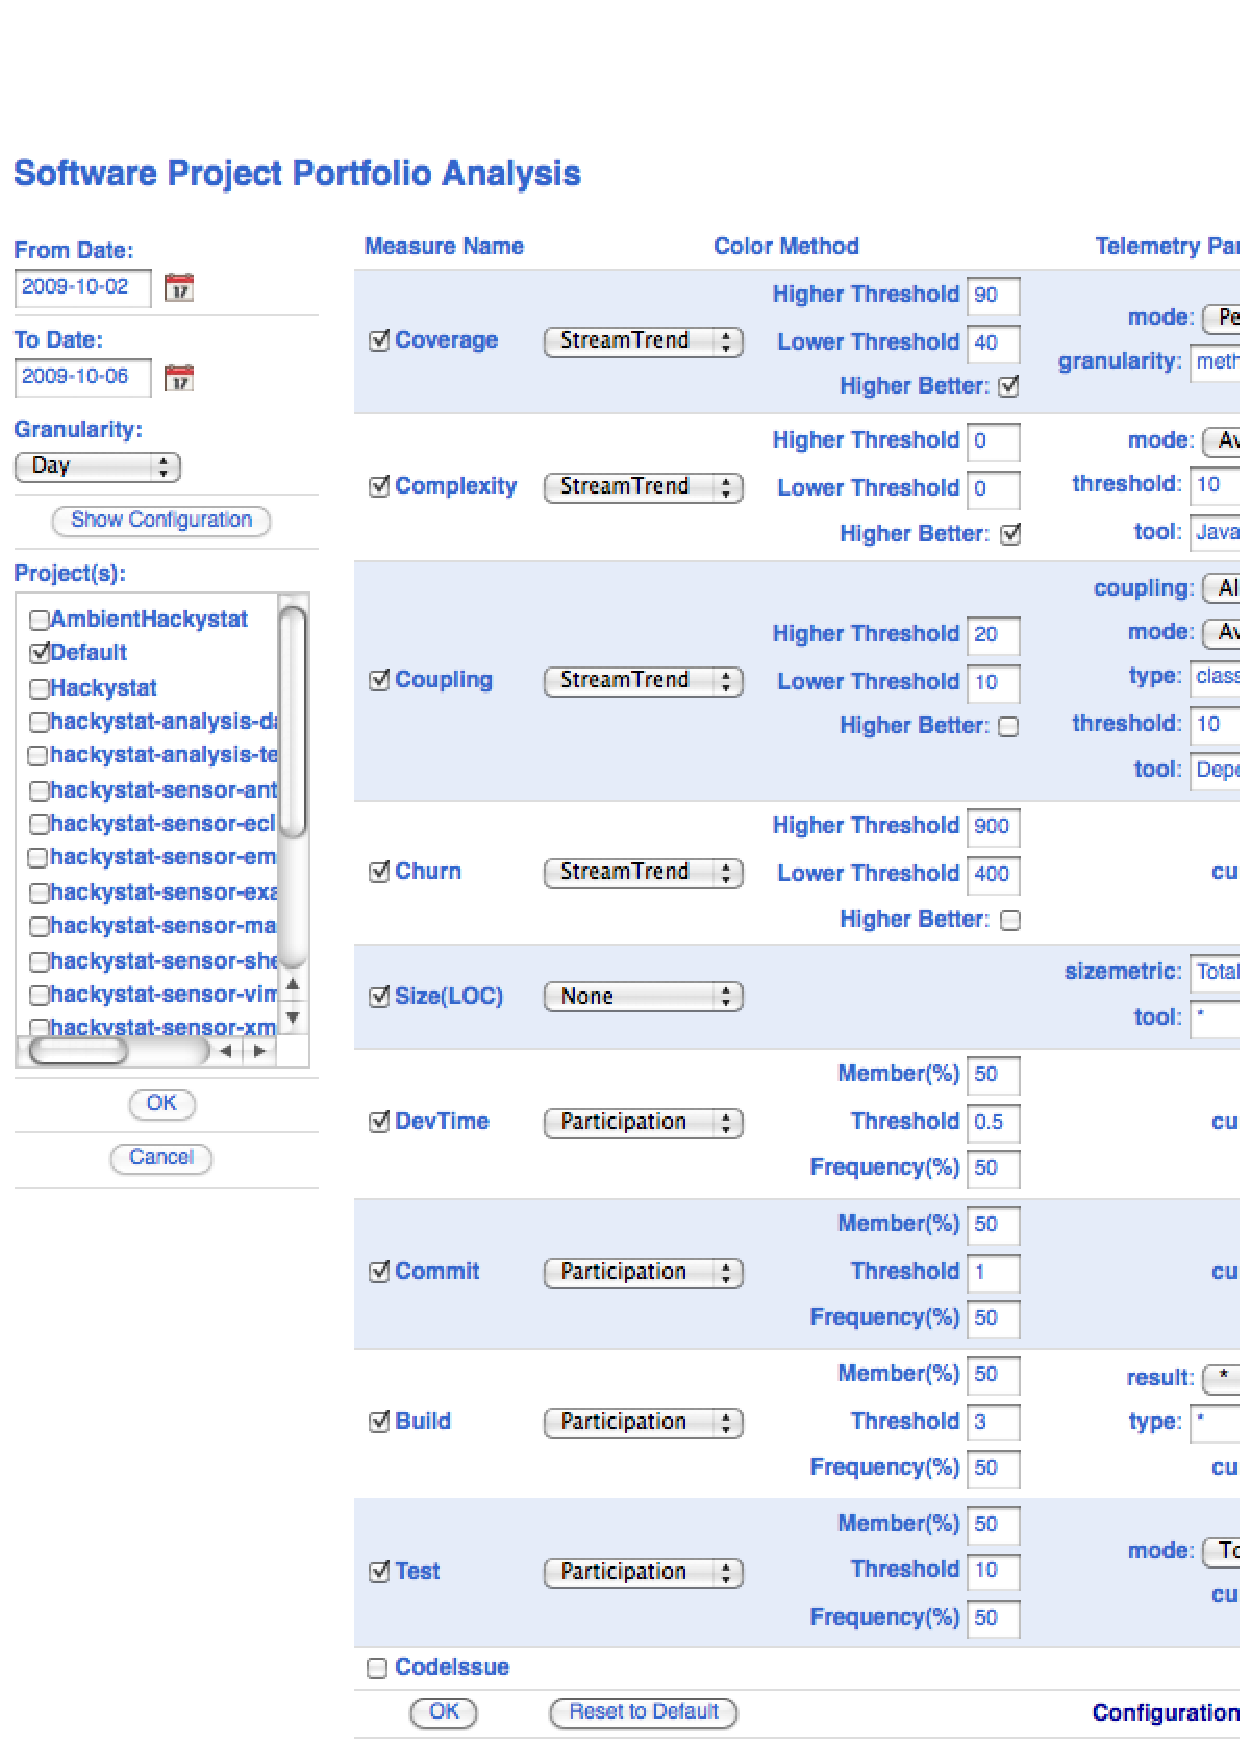
\includegraphics[width=\textwidth]{SICU-configuration} 
   \caption{The Vital Sign Configuration panel in Software ICU}
   \label{fig:SICU-configuration}
\end{figure}

By clicking the ``Show Configuration'' button in the input panel on the left, user can open the configuration panel to its right. Then the ``Show Configuration'' will be disabled when the configuration panel is shown. \autoref{fig:SICU-configuration} shows an example of the vital sign configurations. The first column is the name of the vital sign with the checkbox to enable or disable a vital sign. When a vital sign is disabled, the configuration of color method and Telemetry parameters will disappear, however, the settings are not discarded, thus when enabled again, it will be the same as before it was disabled. The second column is the color method. The current version of Software ICU provides three choices: StreamTrend, Participation and None. By choosing the first two, its associated parameters, which are discussed in \autoref{presentation}, are shown next to the drop-down selection field. When ``None'' is selected, nothing will be shown in that space. The last column is the Telemetry parameters, which is defined in the definition of Telemetry charts, and will be directly transferred to Telemetry service when retrieving Telemetry analysis for vital sign presentation. Because of the implementation, the results of enabling/disabling a vital sign and selecting different color method will be saved immediately, but other fields will only be saved when the ``OK'' button in the bottom is pushed. When the ``OK'' button is pushed, the configuration panel will disappear after setting is saved, and the ``Show Configuration'' button will become available again.

In order to persist the user's configuration setting between each visit, the configuration settings are saved in server side using UriCache. UriCache is a wrapper around the Apache JCS system\footnote{``JCS is a distributed caching system written in java. It is intended to speed up applications by providing a means to manage cached data of various dynamic natures.'' --\url{http://jakarta.apache.org/jcs/}}. It is designed to provide an API well suited to the needs of Hackystat services. The vital sign configuration objects are directly cached, under the name of the user. The cache expiration timer is set to 300 days so that it will not easily be expired. But if the cache is expired, the system will use the default setting of the vital signs.

Next to the ``OK'' button is the ``Rest to Default'' button. It will restore all vital sign configuration settings to default, and the result of restoring will be shown and saved immediately. 

In the bottom-right of the configuration panel is a link called ``Configuration Instructions''. When clicked, it will show a simple instruction of the configuration panel in a pop-up window.


\section{System Customization}
\label{SystemCustomization}

Beside the ability to configure vital signs on the fly, Software ICU provide also offline customization of default vital signs. All vital signs, including the default set discussed above, are defined in PortfolioDefinition XML files. There are two place the system will look for these XML files. The first place is inside the package of detail panel of Software ICU, where the default set of vital signs are defined. The other place is ~/.hackystat/projectbrowser/, where ``~'' stands for user's home directory. Here is an example of the definition XML file:

\begin{verbatim}
<?xml version="1.0" encoding="utf-8"?>
<PortfolioDefinitions>
  <Measures>
    <Measure name="Coverage" 
             classifierMethod="StreamTrend" 
             enabled="true"
             telemetryParameters="Percentage,method">
         <StreamTrendParameters higherBetter="true" 
                                lowerThreshold="40" 
                                higherThreshold="90"/>
    </Measure>
    <Measure name="MemberDevTime" 
             alias="DevTime" 
             merge="sum" 
             classifierMethod="Participation" 
             enabled="true">
          <ParticipationParameters memberPercentage="50" 
                                   thresholdValue="0.5" 
                                   frequencyPercentage="50"/>
    </Measure>
    <Measure name="FileMetric" 
             alias="Size(LOC)" 
             enabled="true">
    </Measure>
  </Measures>
</PortfolioDefinitions>
\end{verbatim}

There is a root element called {\it PortoflioDefinitions}, enclosing a single element {\it Measures}. Within the {\it Measures} element, there are a set of {\it Measure} element, each of which stands for a vital sign. Each {\it Measure} element can take up to six attributes:
\begin{enumerate}
\item The {\it name} attribute is required. It is the name of the Telemetry analysis used in this vital sign.
\item The {\it alias} attribute is optional. When it is set, it will be used as the name of this vital sign. Otherwise, the {\it name} attribute will be used as this vital sign's name.
\item The {\it classifierMethod} attribute defines the default coloring method, either StreamTrend or Participation. This attribute is optional. When it is unset, the default coloring method will be none.
\item The {\it enabled} attribute defines if the vital sign is enabled by default. If set to false, the vital sign will be disabled by default. But the user is still able to enable it in configuration panel.
\item The {\it merge} attribute defines the method to integrate multi-stream telemetry. It is necessary for member-level telemetries to work. ``sum'', ``min'' and ``max'' are available choices. If it is unset, the first stream of the telemetry will be used. Because of the order of streams in a multi-stream telemetry is not guaranteed, using member-level telemetry without setting this attribute might cause unexpected result.
\item The {\it telemetryParameters} attribute is the Telemetry parameters of the telemetry analysis defined in {\it name} attribute. It can be unset, then the default parameters will be used. This attribute accept value formatted the same way as the Telemetry Rest API, i.e. common separated values ordered the same as parameter definition in the Telemetry analysis.
\end{enumerate}

The {\it Measure} element also can have up to two optional sub-elements. They are {\it StreamTrendParameters} and {\it ParticipationParameters}, each of which defines default parameters of the corresponded coloring method, and can exist together regardless what is set in the {\it classifierMethod} attribute. They take the same attributes as their parameters discussed in \autoref{presentation}.

%\section{Permalink supported in Software ICU}
%Permalink support is another important feature that Software ICU provided. A permalink, or permanent link, is a URL that points to a specific page in Internet, i.e. every time users open the same link, they will get the same page. This is especially useful to bookmark a certain analysis or to share an analysis with someone else. Another usage of this feature is that user can directly assemble the URL to achieve an analysis without going over the control panels to get it. 

%An example of a Software ICU's permalink is http://dasha.ics.hawaii.edu:9879/ projectbrowser/ projectportfolio/ 2009-10-02T00:00:00.000-10:00/ 2009-10-06T00:00:00.000-10:00/ Day/ Default::sz@hawaii.edu, hackystat-ui-wicket::randycox@hawaii.edu/.

\chapter{Classroom Evaluation}
This chapter discusses the evaluation of the Software ICU. 

\section{Case Study in Classroom}
The evaluation of the research hypotheses in this project occurred in an academic environment by undergraduates in a senior-level Software Engineering course (ICS 413) at the University of Hawai’i. The class consisted of nineteen students. They were gradually introduced to software engineering concepts like specification, modeling, analysis, and design, along with useful tools including the Eclipse IDE, the JUnit testing framework, the Subversion configuration management system, the Ant build system, and the Hackystat system. As part of the first 7 weeks, they were guided to the three prime directives of open source software (1. The system accomplishes a useful task. 2. An external user can successfully install and use the system. 3. An external developer can successfully understand and enhance the system.), and practiced on these directives on individual basis. Then they were divided into groups of two to work on open source projects hosted on Google Project Hosting, using Subversion system for another 3 weeks. Then Hackystat and the Software ICU were added to their practice. They continued to work on their projects in large size of groups for approximately 5 weeks.

At the end of the Fall 2008 semester, the students in ICS 413 were asked to respond to a questionnaire soliciting their opinions regarding Hackystat and the Software ICU. The complete questionnaire can be found in \autoref{appx:survey}. 

In order to eliminate the potential bias that due to the attempt, either consciously or unconsciously, to "please" the instructor/designer who would presumably be gratified by positive responses to the questionnaire, responses were provided anonymously to the course instructors. It is done in this way: Before the questionnaire is given out, I provided each of the students a ``secret'' code. The correspondence between the secret codes and the students are only known by me, but not the instructor of the class. Response was optional, but the students were offered extra credit points for providing their opinions. The list of names who should be awarded extra credit was sent to the class instructor without identifying individual responses. Eighteen out of the nineteen students contacted provided responses. 

In addition to the survey, I also logged students' activities on Software ICU and the related Telemetry page of Project Browser. Every time when students run an analysis on Telemetry or Software ICU, the name of the analysis, its parameters, and the timestamp of the request is recorded in the log file. I also record the event of clicking the mini chart to run Telemetry drill-down analysis, so that I can assess the drill-down feature is actually useful. The last event I track is changing the configuration of vital signs. However, no meaningful action of configuration is record. This is reasonable because of their lack of sophistication regarding software measurement at the time of the study.

At the end of the evaluation, the log data was compared to the feedbacks from the survey to help verify students responses.

\section {Experimental Limitations}

It is important to recognize the limitations of this study. Compared to the limitations associated with previous study in 2003 and 2006, anonymity is achieved, but others are still unsolved in class evaluation.

First, this data is drawn from a limited sample size of 18 students. The subjects therefore have a relatively narrow and homogeneous background in software development.

Second, the context in which they used the system was a course project.  Course projects tend to be smaller, narrower in scope, and with less pressure on the developers than an industrial context.  It is one thing to get a poor grade for doing a poor job, it is another thing to lose your job for doing a poor job.  In addition, students are not working full-time on the system; the development project is just one assignment among several.  

These are all major limitations on the external validity of the responses.  They do not make the results meaningless, but rather help provide a perspective on how to gain additional evidence in future that would confirm/disconfirm these initial findings.  For example, it would be helpful to deploy Hackystat in a real software company, and then gather data anonymously from the coders and managers. Other insights into future research directions will be covered in an upcoming section.

\chapter {Results}

The results of the classroom evaluation questionnaire can be found in \autoref{appx:result}

\section {Feedback regarding Hackystat system}
Besides the purpose of research regarding Software ICU, this study can also be interpreted as a evaluation of Hackystat's new service oriented architecture.

The responses of the questionnaire indicate that sensors installation is more difficult than Hackystat in 2006. This is not surprising because of the fact that a client-side installer package was provided in 2006, which is not yet available in the time of this study. However, once the sensors are installed correctly, no further effort is required in data collection. Because all the students are using the public services of Hackystat\footnote{SensorBase:\url{http://dasha.ics.hawaii.edu:9876/sensorbase}, DailyProjectData:\url{http://dasha.ics.hawaii.edu:9877/dailyprojectdata}, Telemetry:\url{http://dasha.ics.hawaii.edu:9878/telemetry}, ProjectBrowser:\url{http://dasha.ics.hawaii.edu:9879/projectbrowser}}, there is no effort required in the server-side configuration, which is reported to be the biggest installation/configuration difficulty in Hackystat case study in 2006.

The sensors' installation difficulties is mainly cause by the documentation. Though installation guides are provided for every component, the documentation is too distributed to follow as a result of Hackystat's service-oriented architecture, which reduced the coupling among components, but also reduced the correspondence among components' documentation.

Regarding development data sharing, most students felt OK sharing development data with other members. But three students had concerns that sharing development data would reveal their programming habits and introduce too much competition of statical stats, which made them nervous. It is interesting that those three students are the three with least Software ICU running count in \autoref{fig:per-student-all}. It is reasonable to infer that they worked less harder than other students and did not want to be noticed. However, this is an example of how measurement dysfunction might cause negative effect on developers.

\section {Verification of System Usage}

\autoref{fig:analysis-pop} and \autoref{fig:per-student-all} show the data from system usage logging. I combine it with the data from questionnaire to confirm that the students' responses from questionnaire are reflecting the truths of their practice. 

\begin{figure}[htbp] %  figure placement: here, top, bottom, or page
   \centering
   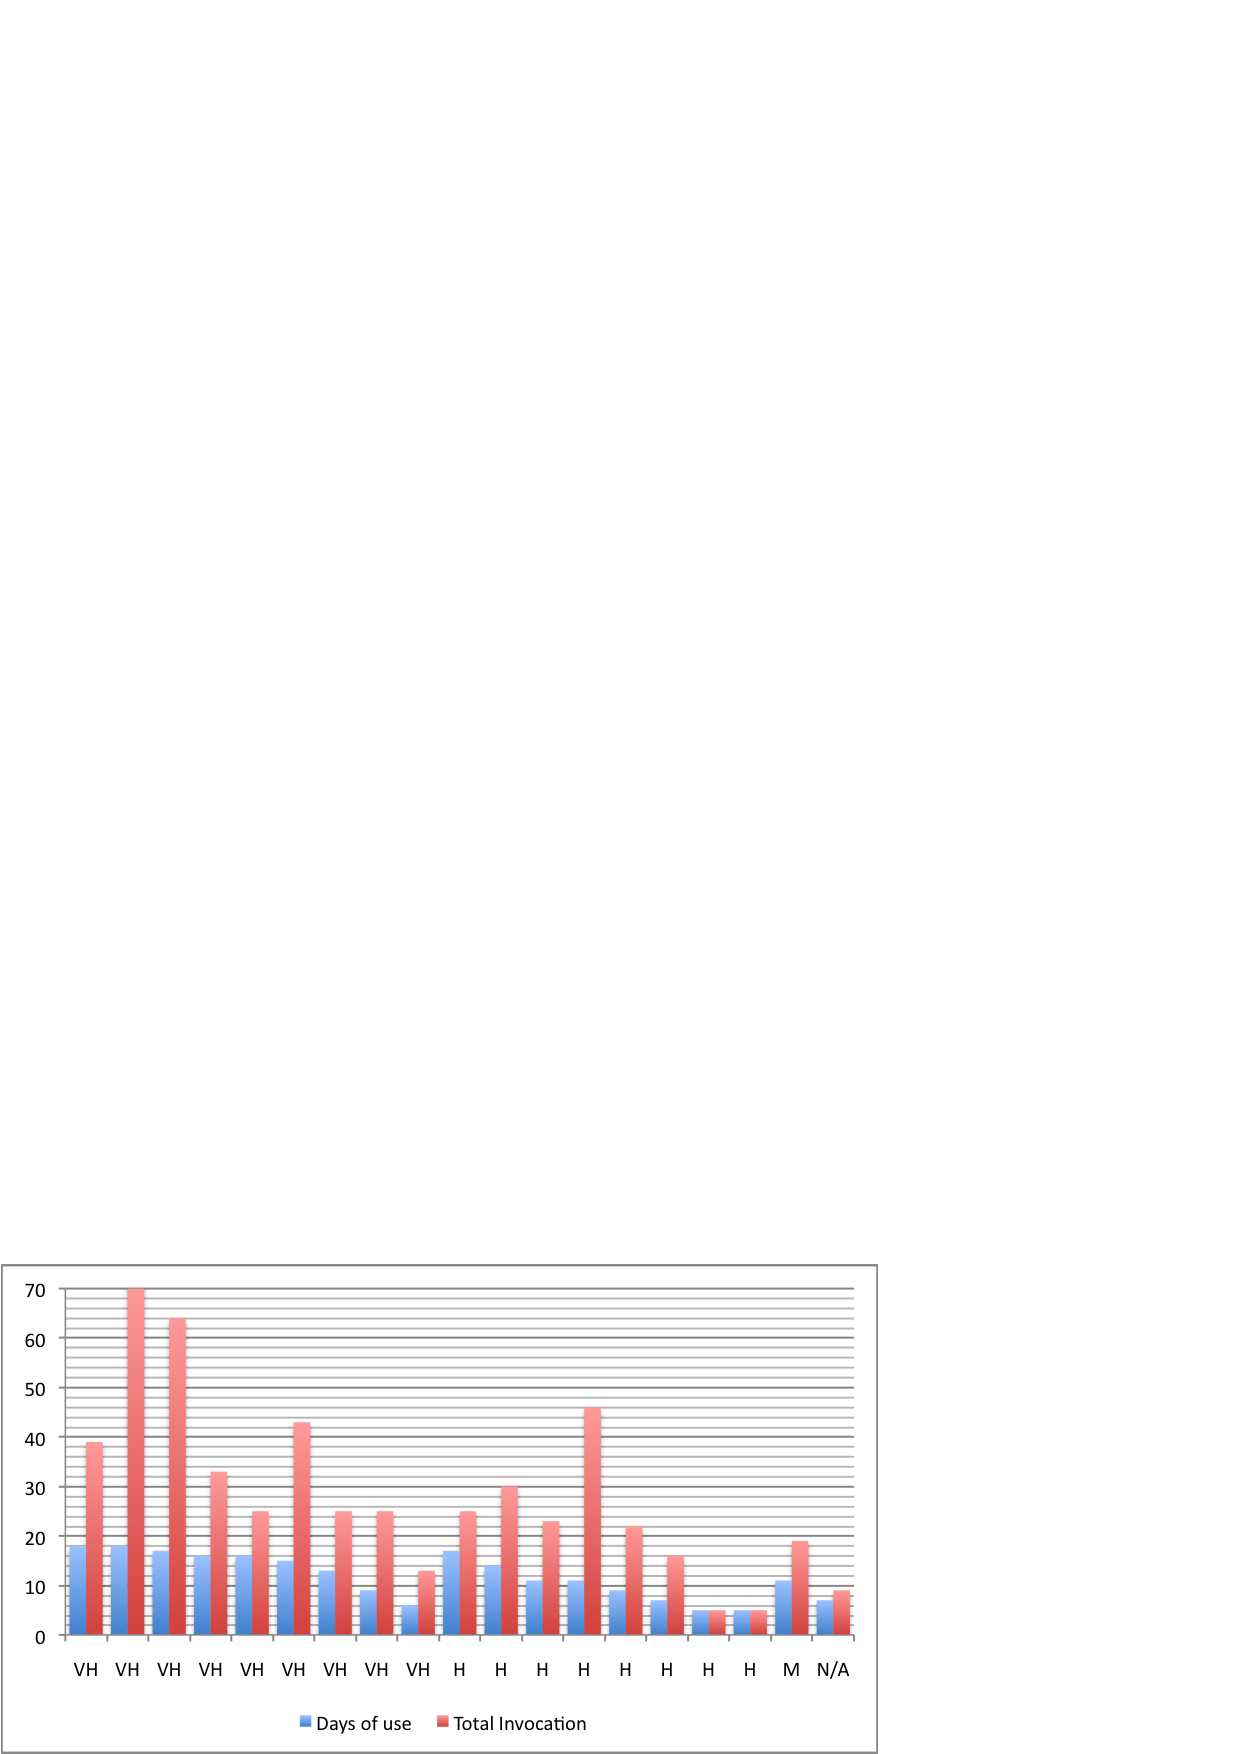
\includegraphics[height=20em]{sicu-usage-verification} 
   \caption[SICU usage on per student bias]{The count of days when SICU was used along with the total invocation on per student bias. Each pair of columns represents data of one student. The X axis shows the responses from questionnaire. VH = every day or more; H = 2-3 times per week; M = once a week; N/A = not available.}
   \label{fig:sicu-usage-verification}
\end{figure}

When verifying the questionnaire responses against the log data, we find that the choices of question ``How frequently did you use the telemetry page? '' and ``How frequently did you use the Software ICU?'' are somehow ambiguous. Though ``every day or more'' is surely asking how many days you use the analysis, ``2-3 times a week'' may be understood as times of invocations. \autoref{fig:sicu-usage-verification} shows data of these two interpretations. If we consider the answers as ``days of use'', the actual use frequencies are much lower than reported, because there are 28 days in the evaluation period but the highest number of days of use is only 18. But if we consider the answers as ``times of invocations'', the invocation frequencies are more matched to reported frequencies. However, in either case, the difference of actual usage between students who claim to use SICU analysis ``every day or more'' and ``2-3 times a week'' is not obvious. Though the total invocation times and days of the first group is higher than the second, some students of the second group used SICU analysis more frequently than the students of the first group. But this error is acceptable because the frequency of use is just as remembered and might not be precise. So if the criteria is weakened and both ``every day or more'' and ``2-3 times a week'' are considered as ``did use SICU frequently'', all responses match their log data except three of them. Those three students claimed that they use Software ICU 2 to 3 times a week or more, but actually only half as much as they claimed (The lowest one with response ``every day or more'' and the lowest two with response of ``2-3 times per week'').

\begin{figure}[htbp] %  figure placement: here, top, bottom, or page
   \centering
   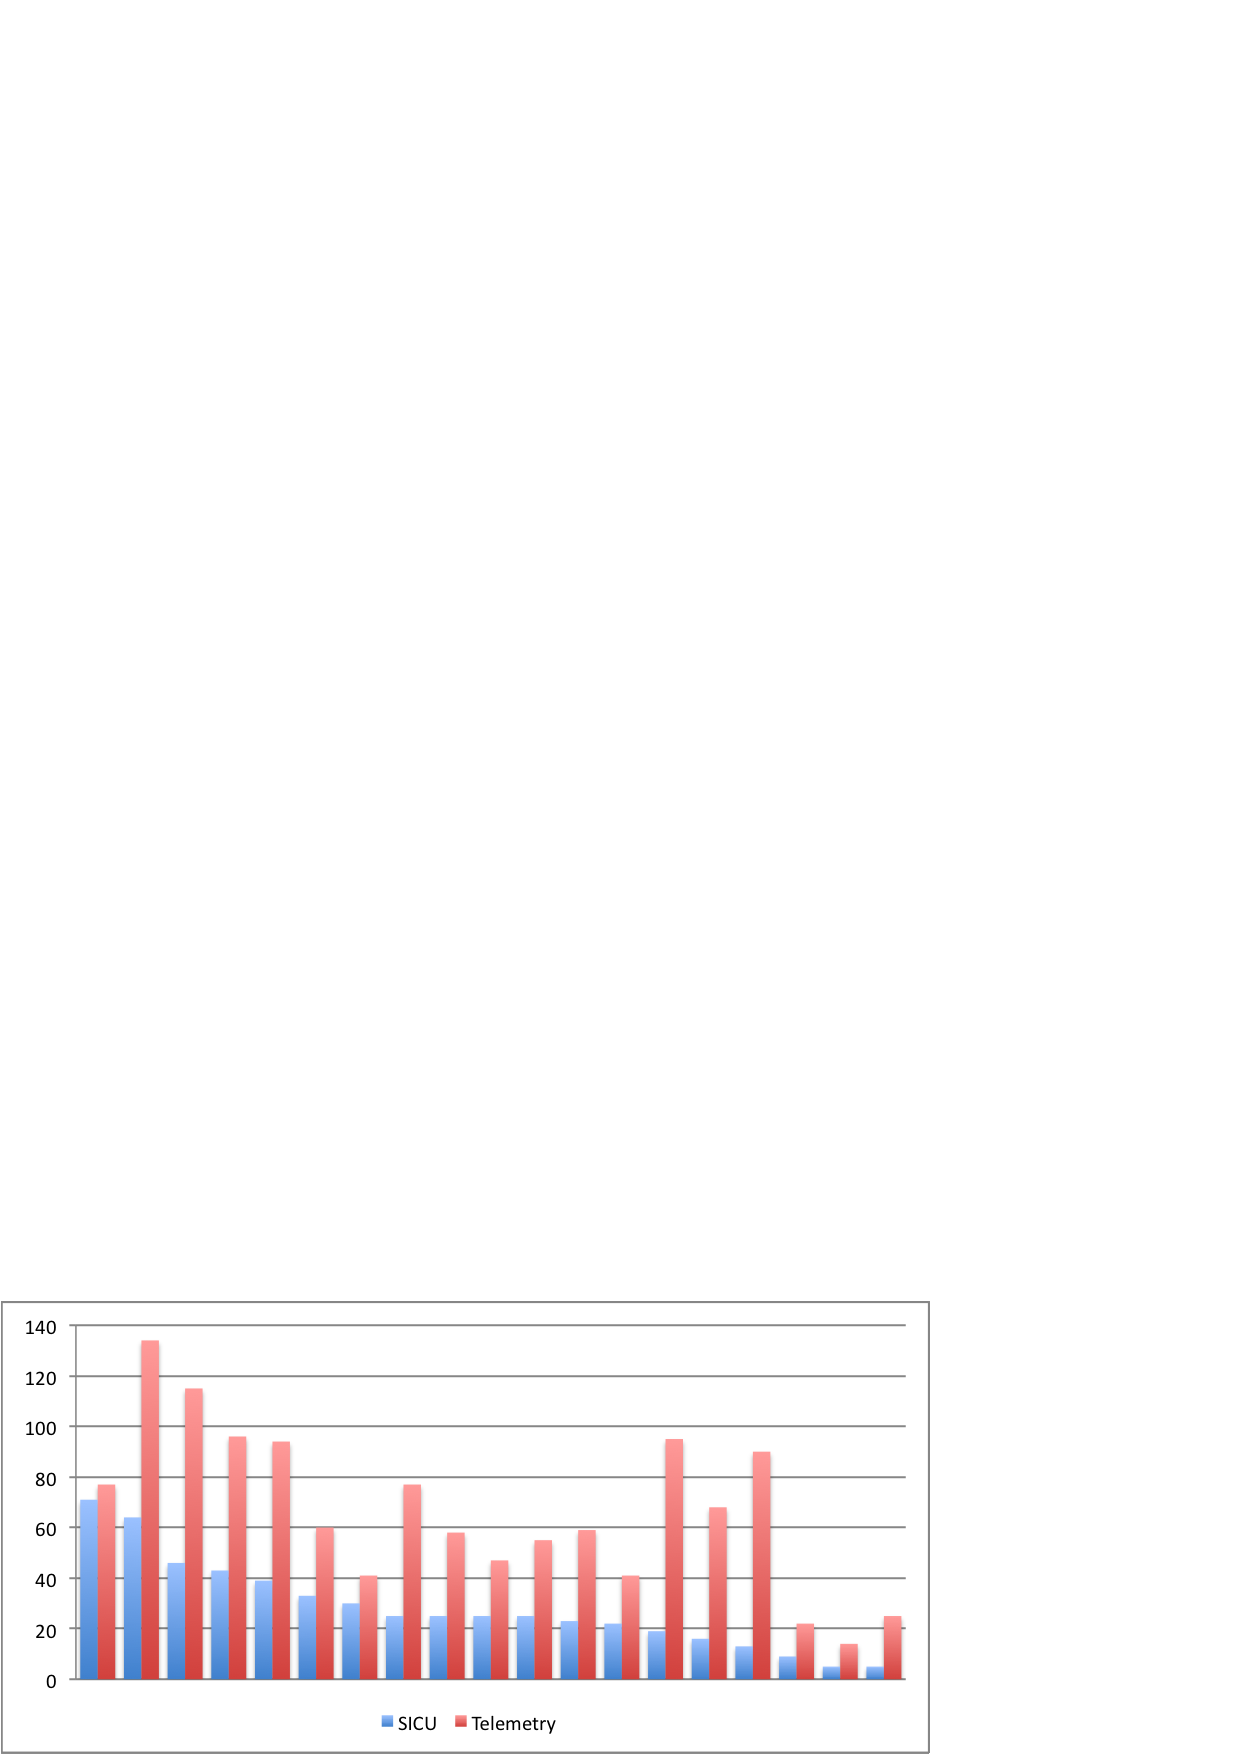
\includegraphics[height=20em]{per-student-all} 
   \caption[Analysis count on a per-student basis]{Analysis count on a per-student basis during the evaluation period. Each pair of columns represents data of one student.}
   \label{fig:per-student-all}
\end{figure}

I also find that though the reported frequency of SICU and Telemetry are similar, Telemetry's analysis invocations are much more than SICU's(see \autoref{fig:per-student-all}). But this matches the native of these two analyses: SICU shows the overall summary of a project's health and no need to run more than once a day, while Telemetry shows detail of a vital sign and would often be run multiple times in every use. 

Because both questionnaire responses and log data show matched evidence that students are using Software ICU and other Hackystat services frequently, I believe that students participated in this evaluations actually have plenty of use experience with the Software ICU and Hackystat and the responses of the questionnaire are based on their real experience and opinions. 

\section{Utilities of Vital Signs}

\begin{figure}[htbp] %  figure placement: here, top, bottom, or page
   \centering
   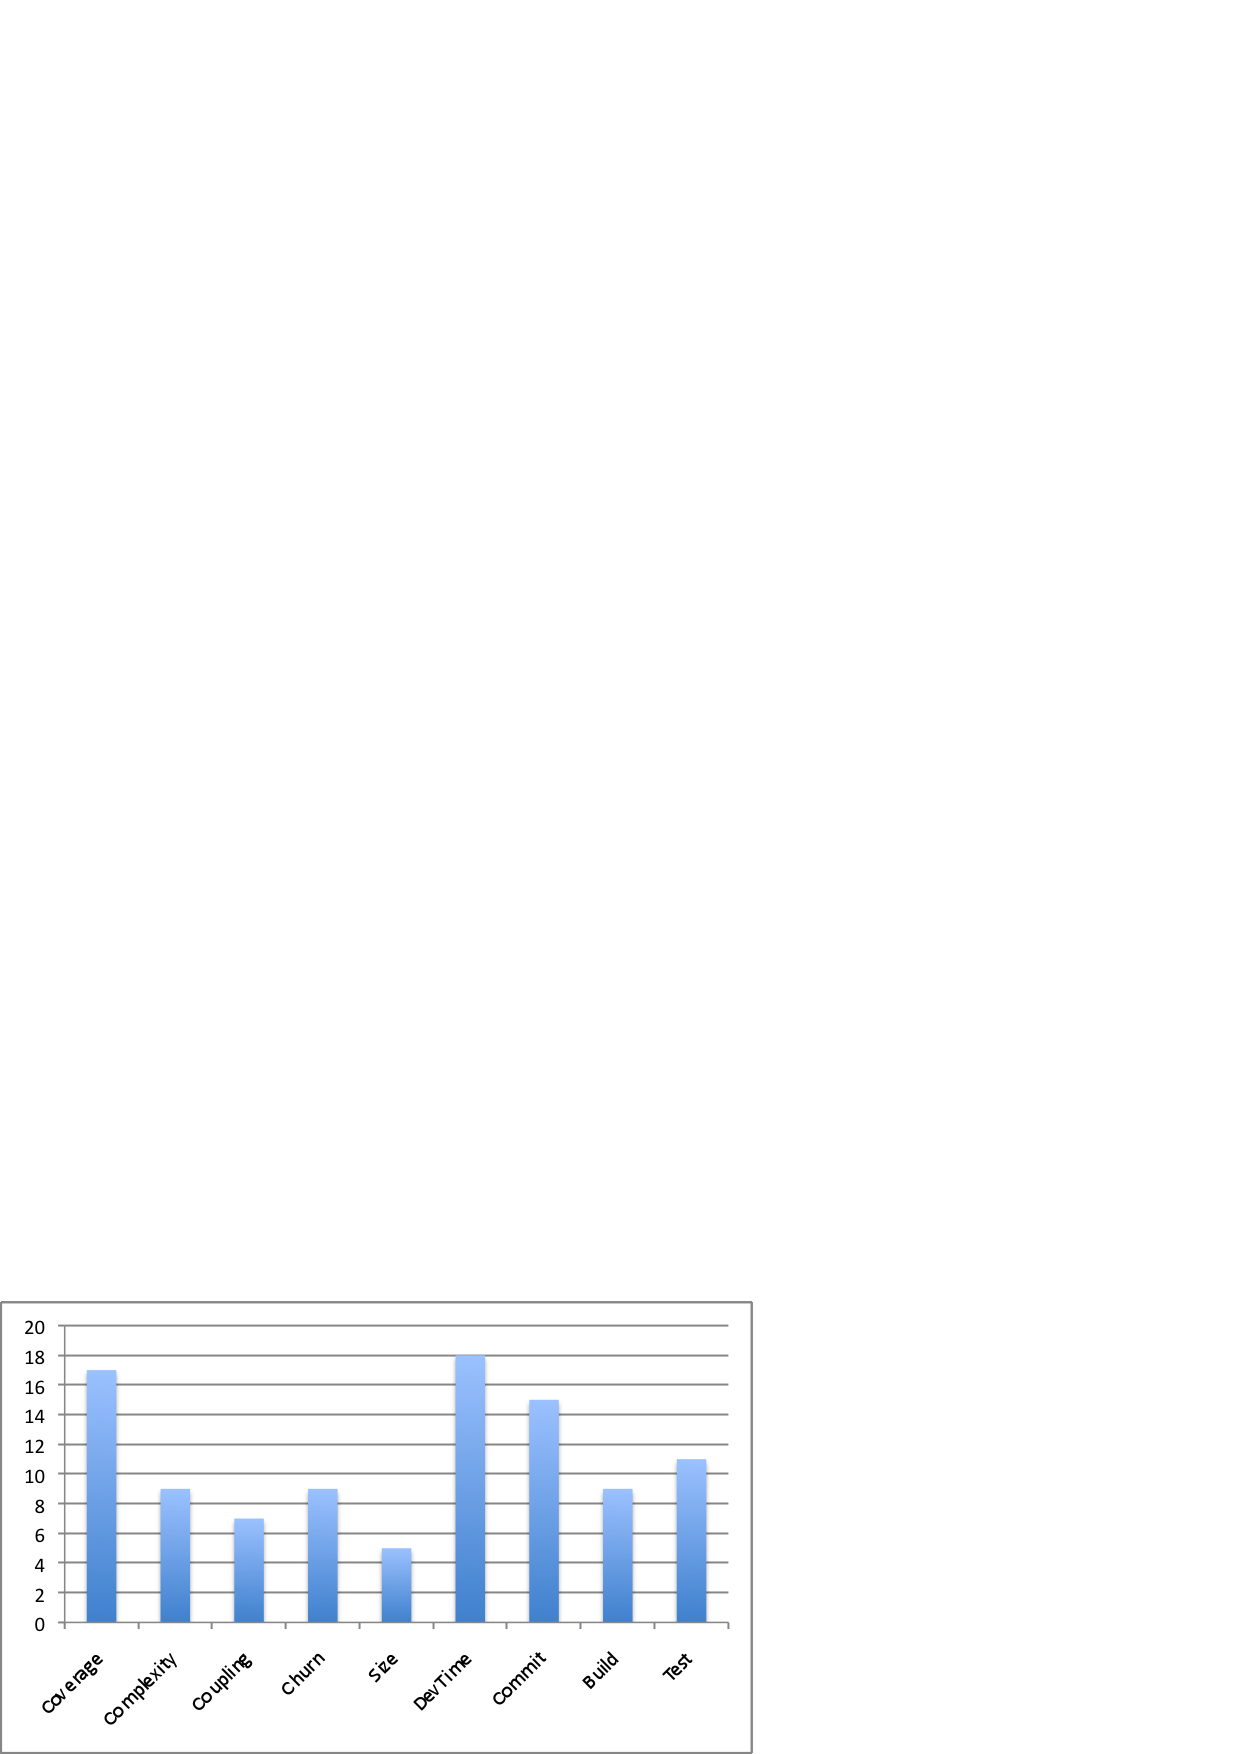
\includegraphics[width=\textwidth]{Q12-UsefulVitalSigns} 
   \caption[Vital sign popularity from survey]{Counts of selections of each vital sign in responses of question ``If you used the Software ICU, please check the vital signs that were useful to you.''.}
   \label{fig:vitalsign-pop}
\end{figure}

Regarding Software ICU as a whole, 7 out of 9 vital signs are considered to be useful by at least half of the respondences (\autoref{fig:vitalsign-pop}). 10 out of 18 responses said Software ICU was accurately reflecting the health of their project via colors. Other 6 responses are not denying the utilities of vital signs, but are arguing that some vital signs are not accurate enough to determine a project's health. Only one student found it is ``hard to determine what will fall into green, red, or yellow'', and the last student said he failed successfully configure the sensors. Overall, students were quite positive regarding the utilities of vital signs.

\begin{figure}[htbp] %  figure placement: here, top, bottom, or page
   \centering
   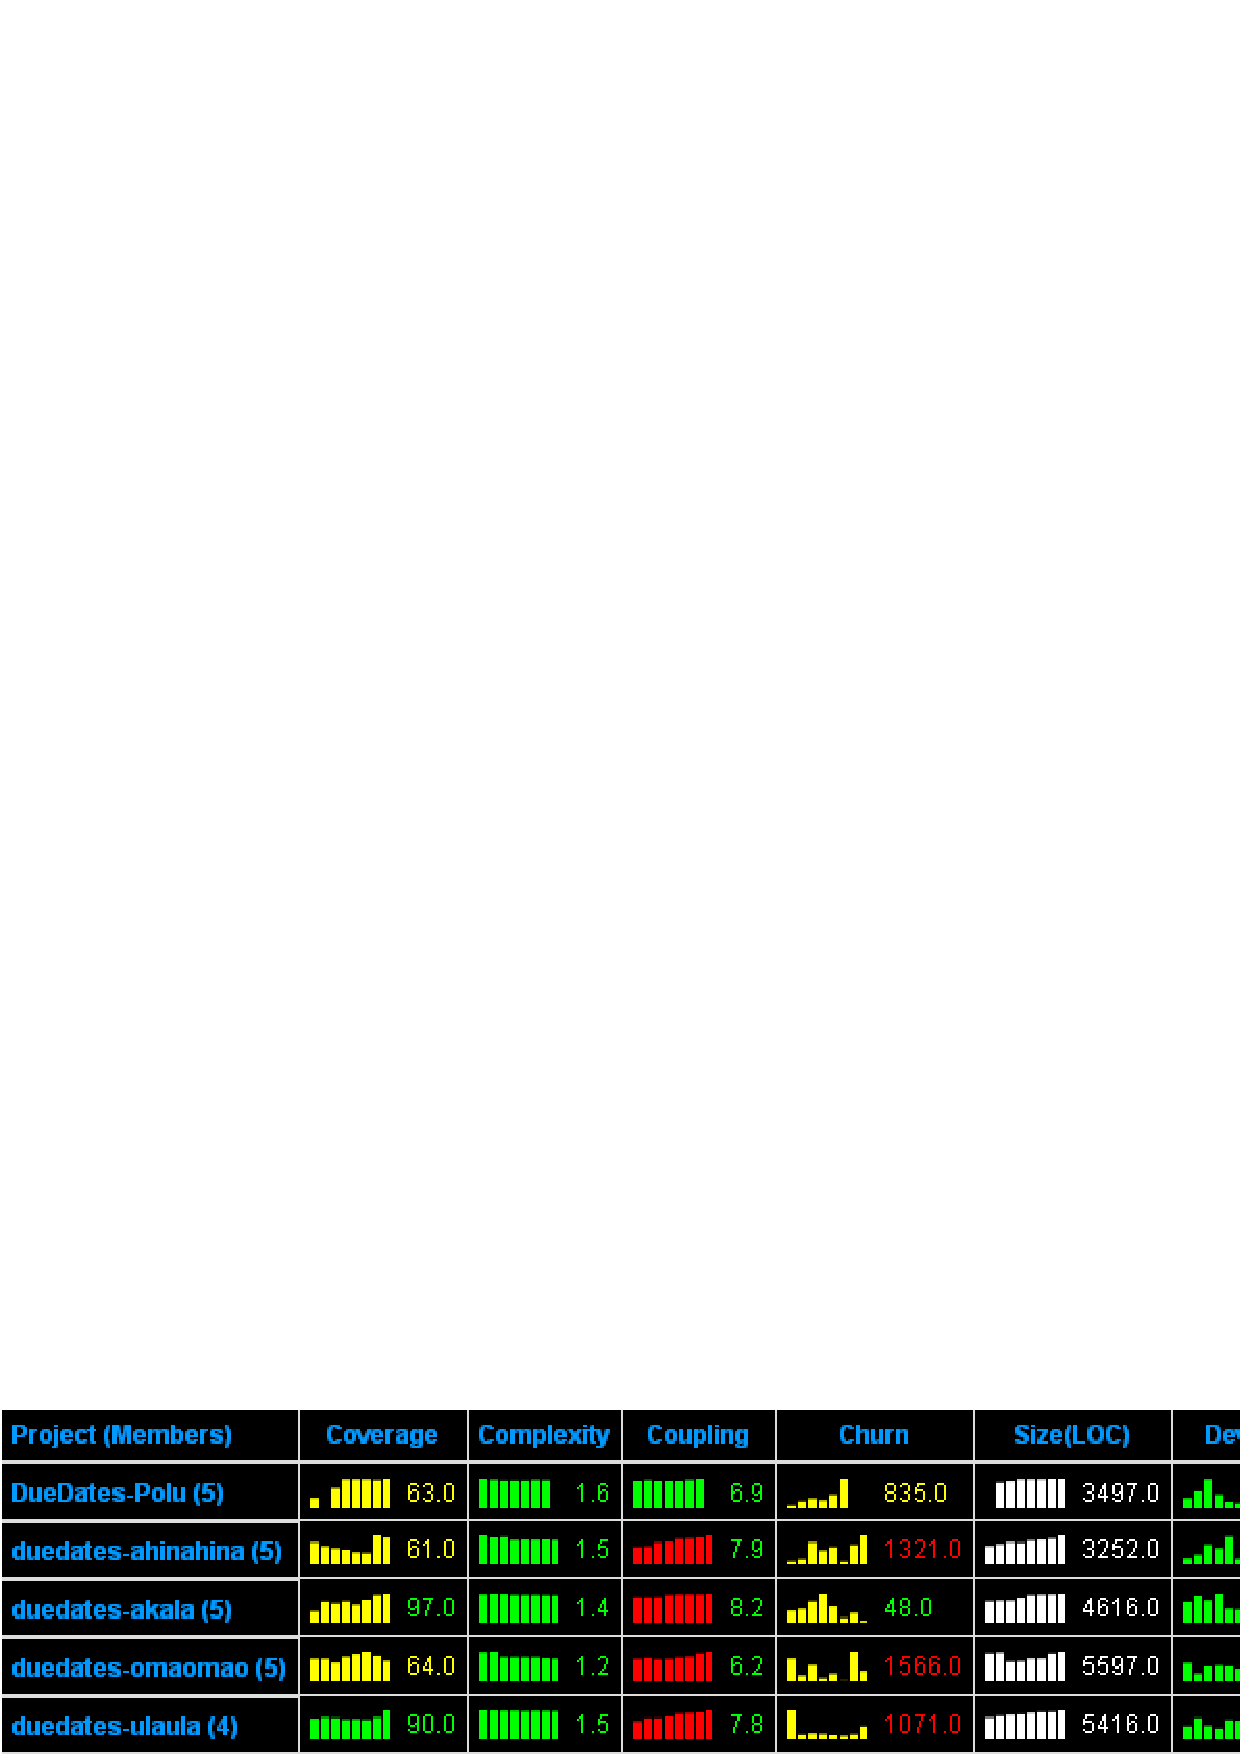
\includegraphics[width=\textwidth]{portfolio-2008} 
   \caption{The final states of all class projects in Software ICU.}
   \label{fig:portfolio-2008}
\end{figure}

Three vital signs cause the most concern in student feedback: Coupling, Churn and DevTime.

Coupling cause concern in that its increase during development is unavoidable, at least there is no easy way to avoid, especially when adopting new packages. The course is not focussed on how to design software to avoid significant increase in Coupling, and students were not experienced enough to figure it out by their own. So student felt confused about what to do: adding new classes and packages is necessary to accomplish the tasks, but it will also increase the coupling and make the vital sign to turn red. As shown in the final states of the class projects in Software ICU (\autoref{fig:portfolio-2008}), 4 of 5 projects failed to keep their Coupling trend green. However, considering their other vital signs, they are not necessarily doing worse than the one with green Coupling. On the other hand, this indicates that the presentation of Coupling vital sign does not accurately reflect the true ``health'' state of the projects.  

Churn's concern can be ascribed to misuse of coloring method. As discussed in \autoref{vitalSign}, Churn is preferred to be relatively stable. Neither significant increase or decrease is desirable. However, a proper coloring method is not yet implemented. Setting the default coloring method is set to StreamTrend with {\it HigherBetter} parameter set to false come out to be a mistake. It mislead students to the impression that Churn should be kept lower, which confused students. On second thought, without a coloring method exclusively designed for Churn, even Participation coloring method might be better than StreamTrend because it can better present process vital signs.

The problem of DevTime is its lack of completeness. Because of the limited collection of DevTime sensors, only a few applications are supported by Hackystat, and only one of them is primarily used by students: the Eclipse IDE. The effort on other development activities, such as reading books, researching online, or even pair programming is not collected. Some students felt compelled to do more coding to catch up with their group partners.


\section {Vital Sign Popularity}

\begin{figure}[htbp] %  figure placement: here, top, bottom, or page
   \centering     
   \subfigure[Invocations of each Telemetry analysis]{
          \label{fig:analysis-pop-all}
          \includegraphics[height=.45\textwidth]{metrics}}
   \vspace{.3in}
   \subfigure[Comparison of member-level and non-member-level analyses]{
          \label{fig:analysis-pop-memberlevel}
          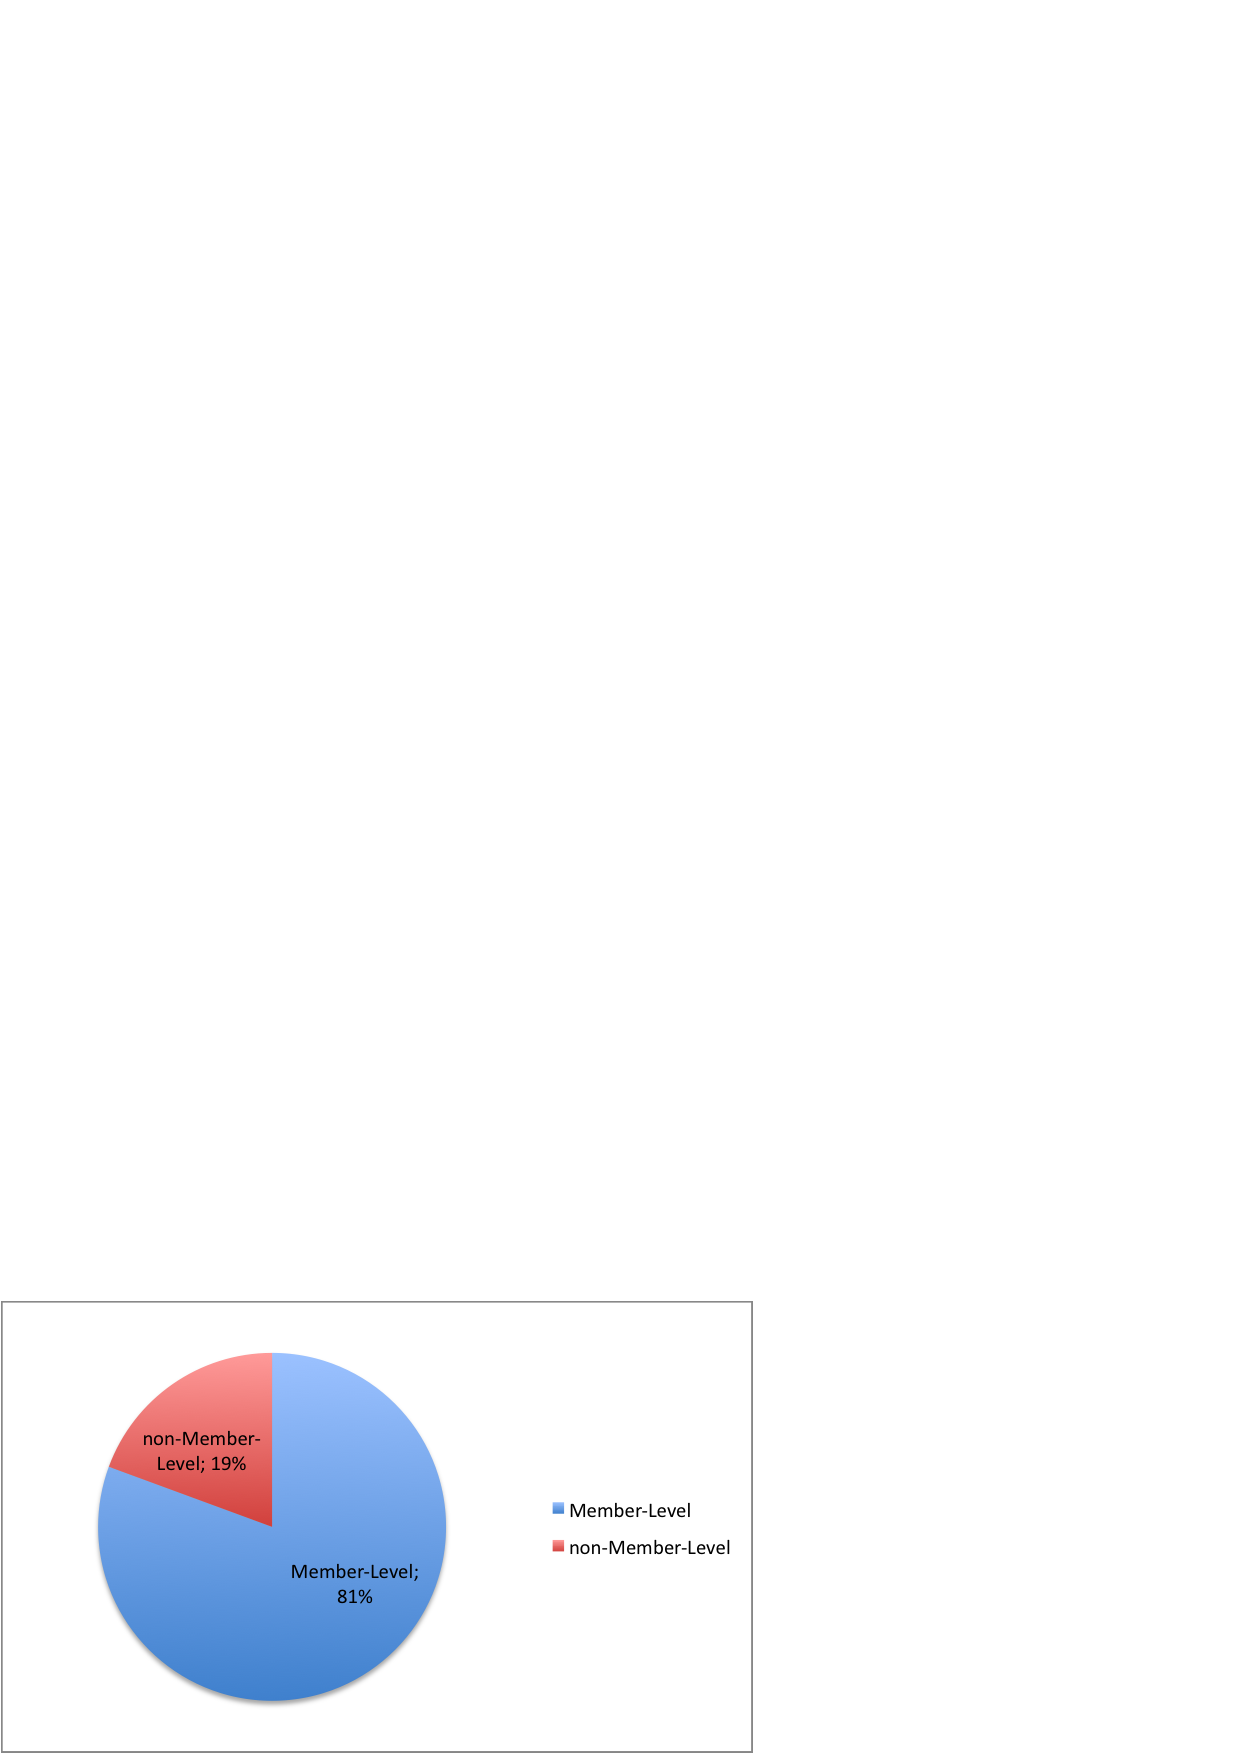
\includegraphics[height=.45\textwidth]{memberlevel}}     
   \caption{Usage of Telemetry Analyses}
   \label{fig:analysis-pop}
\end{figure}

The number of invocations of Telemetry analyses can be an indicator of vital sign popularity and usefulness. Both log data (\autoref{fig:analysis-pop-memberlevel}) and questionnaire responses indicate that Telemetry is mainly used to run member-level analyses. The two most used analyses are MemberDevTime and MemberCommit (\autoref{fig:analysis-pop-all}). In the responses to the question of vital sign usefulness (\autoref{fig:vitalsign-pop}), DevTime and Commit are also among the three most popular vital signs. The other one in the top-three is Coverage. 

It is not surprising that Coverage is among the most popular vital signs. Compared to other productive metrics, it is the most intuitive indicator of project's quality. It is not in the frequently used Telemetry analyses because there is no need to run a separate Telemetry analysis. Users can get all the information from the coverage vital sign in Software ICU.

But DevTime and Commit's popularities were not expected by me prior to the evaluation. Survey result indicates that, this is not a special case: vital signs based on software process metrics attract much more attention than those based on software product metrics (\autoref{fig:vitalsign-pop}). Popularity of process vital signs (DevTime, Commit, Build, Test, and Churn) exceed all productive vital signs except Coverage (Complexity, Coupling and Size). There are three major reasons that lead to this result. 

The first reason is that popular vital signs are much easier to interpret than those that are not popular. The meaning of popular vital signs is very straight-forward. On the contrary, as mentioned in students comments, complexity and coupling metrics are more difficult to comprehend. Though the general guidelines are the lower the better, the meaning of a certain number is not easy to understand because of the nature of these metrics. Also, as the development progresses and more features and functions are added to the code, complexity and coupling always tend to increase. Additionally, unlike coverage that one can simply ``write more tests to increase the coverage'', there is no single obvious way to reduce complexity and coupling. 

Size is an exception because it naturally has no preference to be higher or lower and it is the only vital sign that does not have a default coloring method. It is intended to stay in default vital signs set as a reference rather than an indicator.

The second reason is that productive metrics are less dynamic than process metrics. Productive metrics are statistics of the existed source code. The changes are usually slowly accumulated, so the change of productive metrics are relatively linear. On contrary, process metrics are measurement of human activities, which can vary a lot from day to day. A developer can code for 6 hours in one day but not code at all in the next day. Therefore, the change of process metrics is more interesting.

The last reason, as indicated in students' responses, is because Software ICU is used by some students to improve their team's process by tracking members' activities. As mentioned by a student, member-level Telemetry analyses provide a quantitive way to identify who is falling behind in terms of effort output, thus team members can be more self-critical by comparing their individual data to the groups. Students do make use of these process vital signs to better organize team development. And these vital signs offer a way to motivate students to work hard.

However, one concern is that DevTime and Commit are so popular that they may also induce measurement dysfunctions that affect user's behaviors. As noted by Austin in his Measuring and Managing Performance in Organizations\cite{Austin96}, measurement dysfunction’s defining characteristic is that the actions leading to it fulfill the letter but not the spirit of the stated intentions. At least one student actually experienced this negative effect. He explicitly pointed out that the quantitive measurement of their activities led to a competition of stats within the group. More students have possibly been affected as well because as indicated in that student's answers, his team share the similar opinion of the ``stats competition''.

\section {Feasibility in a professional software development context}
Responses of the questionnaire show that most students thought it was at least somewhat feasible to use Hackystat and Software ICU as a professional developer. Some comments point out some potential barriers of adopting Software ICU to professional setting, including data privacy, data completeness and measurement dysfunctions. But most comments suggest that Hackystat and the Software ICU are useful in professional setting in one way or another.

\section {Thesis Statement Revisited}
With the observations made from the evaluation results, the following summaries can be made about the three hypotheses:
\begin{enumerate}
\item {\it Adopting metaphor of medical ICU to software engineering is practical and feasible.}

The implementation of Software ICU shows abundant evidence to support this hypothesis. Critical functionalities are all implemented at the time of evaluation. Only concerns about implementation from evaluation is the requirement of a choice of emphasized layout that focus  exclusively on single project, which is not difficult to implement at all.
\item {\it The selection of vital signs is appropriate.}

Evidence did suggest that the selected set of vital signs satisfied the need of measurement of the students, and most vital signs were consider useful. However, one concern is that, at the time of study, students' lack of sophistication regarding software measurement may make this conclusion questionable.
\item {\it The coloring mechanism correctly illustrates the health state of the vital signs.}

The result of this is mixed. Firstly, the concept of ``color to state'' is supported from students opinion. Secondly, some vital signs are thought to be correctly colored while some are not. The Participation coloring method enjoyed positive responses on all deployed vital signs, while the StreamTrend coloring method's performance is appropriate on Coverage and Complexity, but is debatable on Coupling and Churn. Lesson from Churn suggest that careful selection of coloring method is as important as development of new one.
\item {\it Knowledge of health state of their projects helps students improve their performance in collaborative software development.}

Comments from questionnaire imply evidence to support this hypothesis. Students stated that the health state of a vital sign guided them to discover and adjust problems in their code or team organization, which will not be (easily) noticed otherwise. But negative impression from inappropriate coloring also affects the conclusion of this hypothesis to some extent. 
\end{enumerate}

\chapter{Conclusions}

\section{Contributions}
This research contributes to empirical software engineering in three ways.

The first contribution is the evidence that Software ICU metaphor and presentation help students understand and utilize software development metrics to improve their individual development performance and team collaboration.

The second contribution of this research is the insight into a new way to teach empirical software engineering course. The classroom case study reveals not only positive impact of the Software ICU paradigm, but also negative affect of measurement dysfunction.

The third contribution of this research is the technical infrastructure, which is open source. Anyone interested can download and use the system in study, teaching or professional development. Software ICU offers not only useful presentation of multiple software development metrics, but also highly configurable and customizable to satisfy various needs. Hackystat is only open source system that provides rich features of automated software engineering measurement and analysis and based on service-oriented architecture, which provide high extensibility. Users can easily configure, modify and/or extend the system according to their special requirements.


\section{Future Direction}
As discussed in previous section, Software ICU still requires more research and improvement to overcome its shortage.

First, vital signs' presentations require more research. The correlation between values of vital signs and the ``health'' state of a project is not yet concluded. Parameters need further tuning to better indicate the ``health'' state of a vital sign. Eventually, more sophisticated vital signs may be needed as well as more sophisticated coloring methods to interpret them. 

Second, it would be interesting to use the Software ICU in an industrial setting. The Software ICU offers powerful means to manage large number of ongoing projects and to fast interpret project ``health'' state, which meets the requirement in project management in industrial environment.
 
Last, but not the least, the completeness of DevTime data awaits further enhancement. The number of applications that are supported by automatic data collection sensors is too small, which may not only impair potential user's motivation of using the system, but also lead to bias in different development activities. This shortage will probably raise the barrier to adopting Hackystat and Software ICU to industry and other software development environment. There are two ways to improve this. The first one is to implement more sensors to more development platform as well as more kinds of development applications. The second one is to provide user a way to manually report development activities, which may be difficult, if ever possible, to capture (e.g. reading paper-based material).


